\documentclass[12pt,a4paper,oneside]{report}

\usepackage[utf8]{vietnam}
\usepackage{mathptmx}
\usepackage{geometry}
\geometry{
    a4paper,
    top=25mm,
    bottom=25mm,
    left=30mm,
    right=20mm,
    headheight=16pt,
    headsep=12pt
}

\usepackage{amsmath,amssymb,amsfonts}
\usepackage{graphicx}
\graphicspath{{../../figures/}{../figures/}{./figures/}{figures/}}
\usepackage{booktabs}
\usepackage{tabularx}
\usepackage{longtable}
\usepackage{array}
\usepackage{float}
\usepackage{setspace}
\onehalfspacing

\usepackage{fancyhdr}
\pagestyle{fancy}
\fancyhf{}
\fancyhead[L]{\small \textsf{Đồ án 1: Trào lưu công suất Newton--Raphson}}
\fancyhead[R]{\small \textsf{ĐHBK Hà Nội -- SEEE}}
\fancyfoot[C]{\thepage}
\renewcommand{\headrulewidth}{0.4pt}
\renewcommand{\footrulewidth}{0pt}

\usepackage{titlesec}
\titleformat{\chapter}[hang]{\bfseries\Large}{\thechapter.\ }{0pt}{}
\titlespacing*{\chapter}{0pt}{-10pt}{15pt}
\titleformat{\section}[hang]{\bfseries\large}{\thesection\ }{0pt}{}
\titleformat{\subsection}[hang]{\bfseries\normalsize}{\thesubsection\ }{0pt}{}

\usepackage{tocloft}
\renewcommand{\cftchapleader}{\cftdotfill{\cftdotsep}}

\renewcommand{\contentsname}{Mục lục}
\renewcommand{\listfigurename}{Danh mục hình vẽ}
\renewcommand{\listtablename}{Danh mục bảng biểu}
\renewcommand{\bibname}{Tài liệu tham khảo}
\renewcommand{\figurename}{Hình}
\renewcommand{\tablename}{Bảng}

\usepackage{xcolor}
\usepackage{hyperref}
\hypersetup{
    colorlinks=true,
    linkcolor=black,
    citecolor=black,
    urlcolor=blue
}

\begin{document}

% ==================== TRANG BÌA CHÍNH (100% TIẾNG VIỆT) ====================
\begin{titlepage}
\begin{center}
    {\large \textbf{ĐẠI HỌC BÁCH KHOA HÀ NỘI}}\\[3pt]
    {\large \textbf{TRƯỜNG ĐIỆN - ĐIỆN TỬ}}\\[3pt]
    {\large \textbf{BỘ MÔN HỆ THỐNG ĐIỆN}}\\[18pt]

    
\includegraphics[width=28mm]{hust_emblem.png}\\[18pt]

    {\Large \textbf{BÁO CÁO ĐỒ ÁN 1}}\\[6pt]
    {\large \textbf{MÃ HỌC PHẦN: EE3810E}}\\[12pt]

    {\Large \textbf{TÍNH TOÁN TRÀO LƯU CÔNG SUẤT BẰNG PHƯƠNG PHÁP NEWTON--RAPHSON: CƠ SỞ LÝ THUYẾT, PHÂN TÍCH PHẦN TỬ LƯỚI, TÍNH TOÁN THỦ CÔNG VÀ ĐỐI CHIẾU VỚI PHẦN MỀM TRÊN CÁC KỊCH BẢN VẬN HÀNH}}\\[22pt]

    \begin{tabular}{ll}
        \textbf{Sinh viên thực hiện:} & \textbf{Lã Huy Gia Huy} \\
        \textbf{Mã số sinh viên:} & \textbf{202412885} \\
        \textbf{Lớp / Khóa:} & \textbf{EE - E18} \\
        \textbf{Chương trình đào tạo:} & Hệ thống điện và Năng lượng tái tạo - 02 \\
        \textbf{Hệ đào tạo:} & Chương trình Tiên tiến (Elite Program) \\
        \textbf{Email:} & Huy.lhg2412885@sis.hust.edu.vn \\[8pt]
        \textbf{Giảng viên hướng dẫn:} & \textbf{TS. Nguyễn Hoàng Việt} \\
        \textbf{Bộ môn:} & Hệ thống điện, Trường Điện - Điện tử \\
        \textbf{Cơ sở đào tạo:} & Đại học Bách khoa Hà Nội \\
    \end{tabular}

    \vfill
    {\large \textbf{HÀ NỘI, THÁNG 10 NĂM 2026}}
\end{center}
\end{titlepage}

% ==================== CÁC TRANG ĐẦU QUYỂN ====================
\pagenumbering{roman}

% --- PHIẾU GIAO NHIỆM VỤ ĐỒ ÁN ---
\chapter*{Phiếu Giao Nhiệm Vụ Đồ Án 1}
\addcontentsline{toc}{chapter}{Phiếu Giao Nhiệm Vụ Đồ Án 1}

\noindent \textbf{1. Thông tin sinh viên:}
\begin{itemize}
    \item Họ và tên sinh viên: \textbf{Lã Huy Gia Huy} \hspace{2cm} MSSV: \textbf{202412885}
    \item Lớp: \textbf{EE - E18} \hspace{4cm} Khóa: \textbf{K69}
    \item Ngành học: Kỹ thuật Điện \hspace{3cm} Chương trình: Tiên tiến (Hệ thống điện và NLTT - 02)
\end{itemize}

\noindent \textbf{2. Đề tài đồ án:}
\begin{quote}
\textit{"Tính toán trào lưu công suất bằng phương pháp Newton--Raphson: Cơ sở lý thuyết, phân tích phần tử lưới, tính toán thủ công và đối chiếu với phần mềm trên các kịch bản vận hành"}
\end{quote}

\noindent \textbf{3. Giảng viên hướng dẫn:} \textbf{TS. Nguyễn Hoàng Việt} (Bộ môn Hệ thống điện, Trường Điện - Điện tử).

\noindent \textbf{4. Mục tiêu kỹ thuật và phạm vi nghiên cứu:}
\begin{enumerate}
    \item \textbf{Cơ sở lý thuyết & Phân tích phần tử lưới:} Phân tích bản chất toán học của hệ phương trình đại số phi tuyến cân bằng công suất nút trong hệ tọa độ cực; mô hình hóa các phần tử cấu trúc lưới điện (đường dây $\pi$ tương đương có dung dẫn $B_0$, máy biến áp, nguồn phát, phụ tải); thiết lập điều kiện dòng nút theo định luật KCL $\mathbf{I}_{\text{bus}} = \mathbf{Y}_{\text{bus}}\mathbf{U}_{\text{bus}}$; phân loại rạch ròi 3 nhóm nút (SLACK, PV, PQ); phân tích sâu các mô hình phụ tải công suất không đổi (PQ) và mô hình phụ tải phụ thuộc điện áp ZIP (Trở kháng $Z$, Dòng điện $I$, Công suất $P$) khi điện áp $U$ thay đổi.
    \item \textbf{Thuật toán Newton--Raphson:} Nghiên cứu nguyên lý tuyến tính hóa Taylor bậc nhất, cấu trúc ma trận Jacobian $\mathbf{J}$ cấp $(2n - 2 - N_{PV})$ với 4 khối $\mathbf{H}, \mathbf{N}, \mathbf{M}, \mathbf{L}$, dẫn xuất tường minh 8 công thức đạo hàm riêng giải tích không qua vi phân số học, và xây dựng lưu đồ thuật toán giải lặp chuẩn mực.
    \item \textbf{Tính toán thủ công "Hộp trắng" (White-Box):} Thực hiện tính toán thủ công từng bước chi tiết (Casio fx-580VN X) trên lưới truyền tải mẫu 3 nút cho Bước lặp 1 ($m = 0 \to 1$), minh bạch toàn bộ các phép thế số trung gian: dẫn nạp nhánh, ma trận dẫn nạp nút $\mathbf{Y}_{\text{bus}}$, véc-tơ sai lệch công suất, tính 9 phần tử ma trận Jacobian $\mathbf{J}^{(0)}$ và giải hệ đại số tuyến tính tìm bước nhảy hiệu chỉnh.
    \item \textbf{Đối chiếu kiểm chứng với công cụ phần mềm PowerFlow:} Sử dụng ứng dụng phần mềm máy tính để bàn PowerFlow đã có sẵn làm công cụ số học đối chứng khách quan; đối chiếu so sánh 1:1 giữa kết quả tính tay và phần mềm; kiểm chứng tốc độ hội tụ bậc hai đạt sai số vô hạn $\Vert \mathbf{f} \Vert_\infty \le 10^{-10}\text{ p.u.}$; kiểm toán cân bằng công suất toàn lưới.
    \item \textbf{Khảo sát các kịch bản vận hành khi điện áp $U$ thay đổi:} Khảo sát định lượng chế độ cơ sở (Base Case), đáp ứng của hệ thống khi phụ tải biến thiên $80\% \to 120\%$ (hiện tượng sụt áp, đường cong $P-U$, phân tích ứng xử mô hình tải ZIP), và giải pháp bù công suất phản kháng $Q_C = 30\text{ Mvar}$ tại nút tải để điều chỉnh nâng cao điện áp nút đạt chuẩn kỹ thuật $[0.95, 1.05\text{ p.u.}]$ cùng việc cắt giảm tổn thất công suất tác dụng.
\end{enumerate}

\vspace{1.5cm}
\noindent \begin{tabular*}{\textwidth}{@{\extracolsep{\fill}}cc}
    \textbf{GIẢNG VIÊN HƯỚNG DẪN} & \textbf{SINH VIÊN THỰC HIỆN} \\[30pt]
    \textbf{TS. Nguyễn Hoàng Việt} & \textbf{Lã Huy Gia Huy}
\end{tabular*}

\newpage

% --- LỜI CAM ĐOAN ---
\chapter*{Lời Cam Đoan}
\addcontentsline{toc}{chapter}{Lời Cam Đoan}

Tôi xin cam đoan bản báo cáo Đồ án 1 với đề tài \textit{"Tính toán trào lưu công suất bằng phương pháp Newton--Raphson: Cơ sở lý thuyết, phân tích phần tử lưới, tính toán thủ công và đối chiếu với phần mềm trên các kịch bản vận hành"} là công trình nghiên cứu lý thuyết, tính toán thủ công độc lập và phân tích thực nghiệm nghiêm túc của bản thân tôi, dưới sự hướng dẫn khoa học trực tiếp của \textbf{TS. Nguyễn Hoàng Việt} tại Bộ môn Hệ thống điện, Trường Điện - Điện tử, Đại học Bách khoa Hà Nội.

Toàn bộ các bước tính toán thủ công minh bạch từng phép thế số trung gian, quá trình đối chiếu kiểm chứng với công cụ phần mềm tính toán PowerFlow đã có sẵn và các phân tích kỹ thuật trên các kịch bản vận hành trình bày trong báo cáo này đều do tôi tự thực hiện và kiểm tra nghiêm ngặt. Tất cả các tài liệu tham khảo, công thức giải tích kinh điển từ các giáo trình chuyên ngành và các bài báo khoa học quốc tế đều đã được trích dẫn nguồn đầy đủ, rõ ràng theo đúng chuẩn mực liêm chính học thuật của Đại học Bách khoa Hà Nội.

\vspace{1.5cm}
\begin{flushright}
    \textit{Hà Nội, ngày 29 tháng 10 năm 2026}\\[5pt]
    \textbf{Sinh viên thực hiện}\\[30pt]
    \textbf{Lã Huy Gia Huy}
\end{flushright}

\newpage

% --- LỜI CẢM ƠN ---
\chapter*{Lời Cảm Ơn}
\addcontentsline{toc}{chapter}{Lời Cảm Ơn}

Lời đầu tiên, em xin được bày tỏ lòng biết ơn sâu sắc và chân thành nhất tới \textbf{TS. Nguyễn Hoàng Việt}, giảng viên trực tiếp hướng dẫn khoa học cho em trong suốt quá trình thực hiện Đồ án 1. Thầy đã định hướng cho em phương pháp luận nghiên cứu khoa học "Hộp trắng" (White-Box), rèn luyện cho em tư duy phân tích bản chất toán học của hệ phương trình trào lưu công suất phi tuyến, kỹ năng tính toán thủ công tỉ mỉ bằng máy tính Casio và phương pháp đối chứng khách quan với công cụ số học, giúp em hiểu sâu sắc về bản chất vận hành của hệ thống điện.

Em xin trân trọng cảm ơn các thầy cô giáo tại \textbf{Bộ môn Hệ thống điện} và \textbf{Trường Điện - Điện tử (SEEE) -- Đại học Bách khoa Hà Nội} đã truyền đạt cho em những nền tảng kiến thức chuyên môn vững chắc, tạo điều kiện thuận lợi nhất cho em trong học tập và nghiên cứu.

Cuối cùng, con xin gửi lời cảm ơn sâu sắc tới gia đình và bạn bè đã luôn động viên, ủng hộ và đồng hành cùng em trong suốt chặng đường học tập tại Đại học Bách khoa Hà Nội.

\vspace{1.5cm}
\begin{flushright}
    \textit{Hà Nội, ngày 29 tháng 10 năm 2026}\\[5pt]
    \textbf{Sinh viên thực hiện}\\[30pt]
    \textbf{Lã Huy Gia Huy}
\end{flushright}

\newpage

% --- TÓM TẮT ĐỒ ÁN ---
\chapter*{Tóm Tắt Đồ Án}
\addcontentsline{toc}{chapter}{Tóm Tắt Đồ Án}

Bài toán trào lưu công suất xác lập (AC Power Flow / Load Flow) là nền móng cốt lõi trong tính toán chế độ xác lập của hệ thống điện, đóng vai trò quyết định trong công tác điều độ thời gian thực, đánh giá an ninh tĩnh và quy hoạch phát triển lưới điện. Đồ án này tiếp cận bài toán dưới góc nhìn khoa học phân tích chuyên sâu kết hợp phương pháp luận \textbf{"Hộp trắng" (White-Box)}, làm sáng tỏ bản chất vật lý và cấu trúc toán học thay vì phụ thuộc thụ động vào các phần mềm "hộp đen":
\begin{itemize}
    \item \textbf{Cơ sở lý thuyết \& Cấu trúc phần tử lưới:} Phân tích dữ liệu đầu vào lưới; định luật dòng nút KCL; phân loại 3 nhóm nút (SLACK, PV, PQ); phân tích sâu mô hình tải PQ và mô hình phụ tải phụ thuộc điện áp ZIP (gồm trở kháng $Z$, dòng điện $I$, công suất $P$) khi điện áp $U$ suy giảm.
    \item \textbf{Hệ phương trình đại số phi tuyến \& Thuật toán Newton--Raphson:} Làm rõ phương trình cân bằng công suất nút tọa độ cực, ẩn số trạng thái $\mathbf{x} = [\boldsymbol{\delta}; \mathbf{U}]$, nghiệm tối ưu $\mathbf{x}^*$, và các đại lượng đầu ra (công suất nguồn Slack, phản kháng máy phát PV, dòng công suất nhánh $S_{ij}$, tổn thất $\Delta S_{ij}$). Thiết lập ma trận Jacobian $\mathbf{J}$ với 4 khối $\mathbf{H}, \mathbf{N}, \mathbf{M}, \mathbf{L}$, dẫn xuất 8 công thức đạo hàm riêng giải tích và lưu đồ giải lặp chuẩn mực.
    \item \textbf{Tính toán thủ công từng bước minh bạch (Hand Calculation):} Trực tiếp giải bằng tay từng bước cho Bước lặp 1 ($m = 0 \to 1$) trên lưới điện mẫu 3 nút (Nút 1 Slack $1.05\text{ pu}$, Nút 2 PV $1.04\text{ pu}, 50\text{ MW}$, Nút 3 PQ $120\text{ MW} + j50\text{ Mvar}$) bằng máy tính Casio fx-580VN X, thể hiện đầy đủ mọi phép thế số trung gian, ma trận dẫn nạp $\mathbf{Y}_{\text{bus}}$, sai lệch công suất, tính 9 phần tử ma trận Jacobian và giải hệ đại số tuyến tính tìm bước nhảy hiệu chỉnh.
    \item \textbf{Đối chiếu kiểm chứng với công cụ phần mềm PowerFlow:} Sử dụng ứng dụng phần mềm tính toán số học PowerFlow đã có sẵn để thực hiện đối chiếu kiểm chứng 1:1 với kết quả tính tay; kết quả cho thấy độ trùng khớp số học tuyệt đối ở Bước lặp 1 với sai số triệt tiêu $< 10^{-5}$ do làm tròn bấm máy tính tay; phần mềm hội tụ bậc hai hoàn hảo sau 4 bước lặp với sai số vô hạn $\Vert \mathbf{f} \Vert_\infty = 6.22 \times 10^{-15}\text{ p.u.}$, xác định điện áp xác lập nút tải $U_3 = 0.944383\text{ pu}$ và tổng tổn thất tác dụng $\Delta P_{\text{loss}} = 6.4522\text{ MW}$.
    \item \textbf{Khảo sát các kịch bản vận hành khi điện áp $U$ thay đổi:} Khảo sát định lượng đáp ứng của lưới khi phụ tải tăng từ $80\%$ lên $120\%$ dẫn đến sụt áp phi tuyến tại nút tải ($U_3$ giảm xuống $0.9180\text{ p.u.}$, vi phạm ngưỡng vận hành), xây dựng đường cong $P-U$, phân tích ứng xử tự điều chỉnh của phụ tải ZIP; khảo sát giải pháp bù công suất phản kháng $Q_C = 30\text{ Mvar}$ tại nút tải giúp khôi phục điện áp lên $0.9786\text{ p.u.}$ (đạt chuẩn tối ưu $[0.95, 1.05\text{ p.u.}]$) và giảm $16.54\%$ tổn thất công suất tác dụng toàn lưới.
\end{itemize}

\noindent \textbf{Từ khóa:} Trào lưu công suất xác lập, Thuật toán Newton--Raphson, Ma trận Jacobian, Ma trận dẫn nạp nút $\mathbf{Y}_{\text{bus}}$, Dòng nút KCL, Mô hình phụ tải ZIP, Tính toán thủ công Casio, Phần mềm PowerFlow, Đối chiếu kiểm chứng, Đáp ứng điện áp $U$, Bù công suất phản kháng.

\newpage

% --- MỤC LỤC, DANH MỤC HÌNH VẼ, BẢNG BIỂU ---
\tableofcontents
\newpage
\listoffigures
\newpage
\listoftables
\newpage
\pagenumbering{arabic}
\setcounter{page}{1}

% ==================== CHƯƠNG 1: GIỚI THIỆU CHUNG ====================
\chapter{Giới Thiệu Chung Và Bài Toán Trào Lưu Công Suất}

\section{Vai Trò Và Ý Nghĩa Thực Tiễn Của Trào Lưu Công Suất}
Trong kỹ thuật hệ thống điện hiện đại, bài toán tính toán trào lưu công suất xác lập (AC Power Flow / Load Flow) là nền móng cốt lõi trong phân tích chế độ xác lập của lưới điện. Đây là công cụ toán học bắt buộc phải thực hiện đầu tiên trong mọi quy trình kỹ thuật:
\begin{enumerate}
    \item \textbf{Vận hành và điều độ hệ thống điện thời gian thực:} Giúp Trung tâm Điều độ Hệ thống điện Quốc gia và các cấp điều độ miền giám sát trạng thái an ninh của lưới điện, kiểm soát điện áp tại tất cả các thanh cái nằm trong dải cho phép ($0.95 \le U_i \le 1.05\text{ p.u.}$), theo dõi mức độ mang tải của các đường dây truyền tải và máy biến áp, đồng thời điều độ tối ưu công suất tác dụng và công suất phản kháng giữa các nguồn điện.
    \item \textbf{Quy hoạch phát triển hệ thống điện:} Tính toán chế độ trào lưu công suất cho phép các kỹ sư quy hoạch dự báo khả năng đáp ứng của lưới điện trước nhu cầu phụ tải tăng trưởng trong tương lai, xác định thời điểm và vị trí tối ưu để xây dựng thêm đường dây mới, lắp đặt trạm biến áp mới hoặc bổ sung nguồn điện năng lượng tái tạo.
    \item \textbf{Cung cấp điểm làm việc cơ sở cho các bài toán phân tích chuyên sâu:} Cung cấp điểm làm việc tĩnh xác lập phục vụ tính toán ngắn mạch, phân tích ổn định góc công suất (ổn định quá độ), ổn định điện áp tĩnh (phân tích đường cong $P-U$, $Q-V$) và đánh giá an ninh tĩnh $N-1$.
\end{enumerate}

Về bản chất, bài toán trào lưu công suất xác định trạng thái làm việc của mạng điện thông qua véc-tơ biến trạng thái điện áp nút: véc-tơ độ lớn điện áp $\mathbf{U} = [U_1, U_2, \dots, U_n]^T$ và véc-tơ góc pha điện áp $\boldsymbol{\delta} = [\delta_1, \delta_2, \dots, \delta_n]^T$. Sau khi giải ra trạng thái điện áp, mọi thông số vận hành thứ cấp như dòng công suất chạy trên từng nhánh đường dây, công suất phát tại nút cân bằng và tổng tổn thất kỹ thuật toàn lưới đều được xác định trực tiếp thông qua các biểu thức giải tích.

\section{Mục Tiêu Đề Tài Và Phương Pháp Luận "Hộp Trắng" (White-Box)}
Trong thực tiễn đào tạo và nghiên cứu hiện nay, các kỹ sư thường sử dụng các phần mềm thương mại (PSS/E, PowerWorld) hoặc các thư viện mã nguồn mở có sẵn. Tuy nhiên, nếu chỉ sử dụng phần mềm như những "hộp đen" (Black-Box) bằng cách nhập dữ liệu và nhận kết quả, người kỹ sư sẽ không thể nắm bắt được:
\begin{itemize}
    \item Dữ liệu đầu vào của hệ thống điện được cấu trúc và chuyển đổi thành mô hình toán học như thế nào?
    \item Ma trận dẫn nạp nút $\mathbf{Y}_{\text{bus}}$ được tổng hợp giải tích ra sao từ các nhánh đường dây hình $\pi$ có dung dẫn nạp nối đất?
    \item Hệ phương trình đại số phi tuyến cân bằng công suất nút có dạng toán học như thế nào, đâu là ẩn số trạng thái và đâu là điều kiện biên của từng loại nút?
    \item Từng phần tử của ma trận đạo hàm riêng Jacobian được dẫn xuất và tính toán số học qua từng bước lặp như thế nào?
    \item Khi điện áp nút $U$ thay đổi, các mô hình phụ tải khác nhau (PQ và ZIP) tác động ngược trở lại dòng điện nút và trào lưu công suất ra sao?
\end{itemize}

Xuất phát từ yêu cầu học thuật nghiêm cẩn của Bộ môn Hệ thống điện (Đại học Bách khoa Hà Nội), đồ án này không đặt mục tiêu xây dựng một phần mềm mới từ đầu, mà tập trung vào:
\begin{enumerate}
    \item \textbf{Nghiên cứu sâu sắc cơ sở lý thuyết toán học:} Phân tích cấu trúc các phần tử của lưới, dạng phương trình đại số phi tuyến, điều kiện dòng nút KCL, phân loại nút và các mô hình phụ tải (PQ, ZIP).
    \item \textbf{Phương pháp luận "Hộp trắng" (White-Box):} Trực tiếp sử dụng máy tính Casio fx-580VN X để tính toán thủ công từng bước chi tiết cho Bước lặp 1 ($m = 0 \to 1$) trên lưới điện truyền tải mẫu 3 nút, trình bày minh bạch mọi phép thế số trung gian, không bỏ sót bất kỳ bước số học nào.
    \item \textbf{Đối chiếu kiểm chứng 1:1 với công cụ phần mềm PowerFlow:} Sử dụng phần mềm tính toán số học PowerFlow đã có sẵn làm công cụ đối chứng khách quan, khẳng định sự trùng khớp tuyệt đối giữa lý thuyết tính tay và kết quả giải số trên máy tính.
    \item \textbf{Khảo sát các kịch bản vận hành thực tế khi điện áp $U$ thay đổi:} Thực nghiệm đánh giá đáp ứng của hệ thống khi phụ tải thay đổi, kiểm tra hiện tượng sụt áp, phân tích ứng xử của mô hình tải ZIP và hiệu quả của giải pháp bù công suất phản kháng tại nút tải.
\end{enumerate}

\section{Hệ Đơn Vị Tương Đối (p.u.) Trong Tính Toán Hệ Thống Điện}
Trong hệ thống điện thực tế gồm nhiều cấp điện áp liên kết qua các máy biến áp, việc sử dụng các đại lượng có thứ nguyên ($\Omega, \text{kV}, \text{MW}, \text{Mvar}$) khiến hệ phương trình trở nên phức tạp do phải quy đổi trở kháng qua tỷ số biến áp lý tưởng. Hệ đơn vị tương đối (per-unit system - p.u.) giải quyết triệt để vấn đề này bằng cách chuẩn hóa mọi đại lượng theo các giá trị cơ bản:
\begin{equation}
\text{Giá trị (p.u.)} = \frac{\text{Giá trị thực}}{\text{Giá trị cơ bản}}
\end{equation}
Chọn công suất cơ bản 3 pha thống nhất toàn hệ thống là $S_{\text{base}} = 100.0\text{ MVA}$. Điện áp cơ bản $U_{\text{base}}$ được chọn tương ứng với điện áp danh định của từng cấp điện áp (ví dụ cấp truyền tải $110\text{ kV}$). Trở kháng cơ bản $Z_{\text{base}}$ và dẫn nạp cơ bản $Y_{\text{base}}$ được suy ra:
\begin{equation}
Z_{\text{base}} = \frac{U_{\text{base}}^2}{S_{\text{base}}}, \qquad Y_{\text{base}} = \frac{1}{Z_{\text{base}}} = \frac{S_{\text{base}}}{U_{\text{base}}^2}
\end{equation}

% ==================== CHƯƠNG 2: MÔ HÌNH HÓA TOÁN HỌC ====================
\chapter{Cấu Trúc Lưới Điện Và Hệ Phương Trình Đại Số Trào Lưu Công Suất}

\section{Cấu Trúc Lưới Điện Và Các Phần Tử Đầu Vào}
Đầu vào của bài toán trào lưu công suất bao gồm cấu trúc hình học của mạng điện (Topology) và thông số kỹ thuật của các phần tử đấu nối:

\subsection{1. Danh Mục Nút (Bus Data)}
Mỗi nút $i$ trong hệ thống điện đại diện cho một thanh cái (Busbar). Dữ liệu đầu vào của nút bao gồm:
\begin{itemize}
    \item Số hiệu nút $i$ và tên định danh thanh cái.
    \item Loại nút: Nút cân bằng (SLACK), Nút điều áp (PV), hoặc Nút phụ tải (PQ).
    \item Thông số nguồn phát: Công suất tác dụng phát $P_{Gi}$, công suất phản kháng phát $Q_{Gi}$, giới hạn công suất phản kháng $[Q_{Gi}^{\min}, Q_{Gi}^{\max}]$.
    \item Thông số phụ tải: Công suất tác dụng tiêu thụ $P_{Li}$, công suất phản kháng tiêu thụ $Q_{Li}$.
    \item Điện áp đặt trước: Độ lớn điện áp $U_i$ (cho nút Slack và PV), góc pha ban đầu $\delta_i$ ($\delta_1 = 0^\circ$ cho nút Slack).
    \item Dung dẫn nạp bù ngang đặt cố định tại thanh cái: $y_{\text{shunt}, i} = g_{sh, i} + j b_{sh, i}$ (ví dụ tụ bù ngang hoặc kháng bù ngang).
\end{itemize}

\subsection{2. Đường Dây Truyền Tải (Mô Hình $\pi$ Tương Đương)}
Đối với đường dây truyền tải điện áp cao từ trung bình đến dài, điện dung giữa dây dẫn và đất sinh ra dòng điện nạp đáng kể. Đường dây được mô hình hóa chính xác bằng sơ đồ hình $\pi$ tương đương (Hình~\ref{fig:pi_model}):

\begin{figure}[H]
\centering
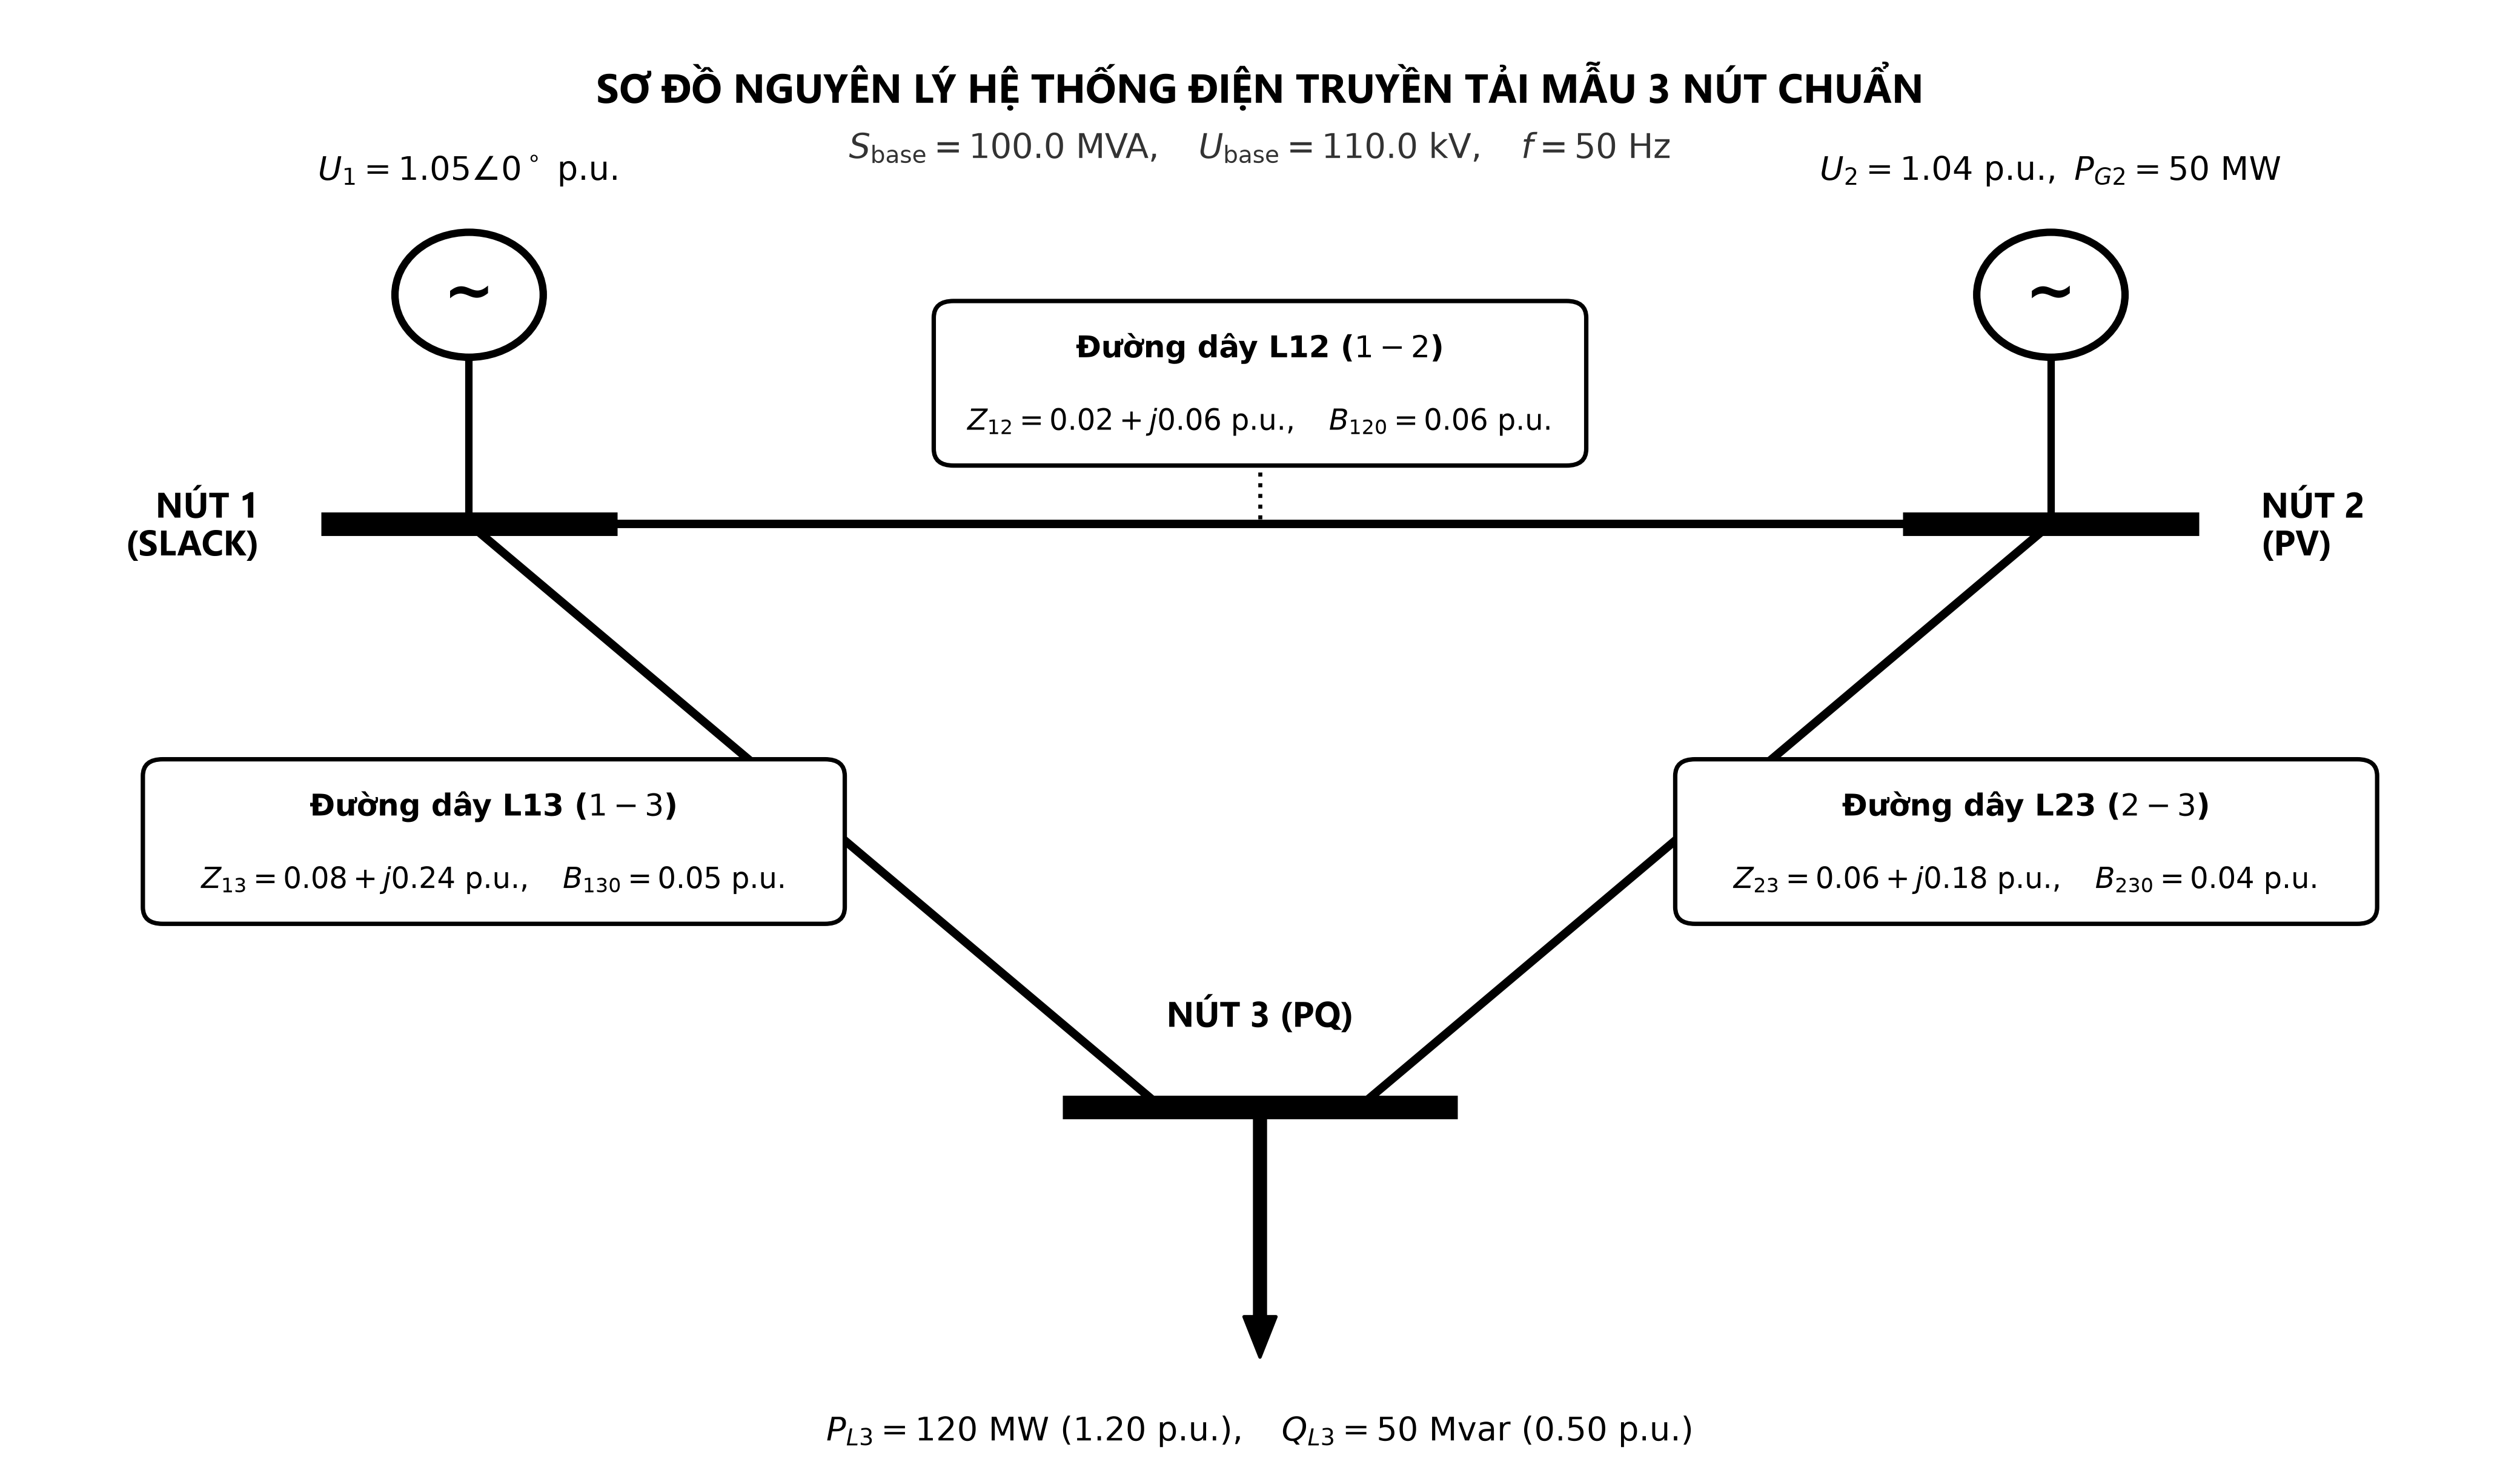
\includegraphics[width=0.65\textwidth]{3bus_network_vi.png}
\caption{Mô hình $\pi$ tương đương và sơ đồ mạng lưới truyền tải mẫu.}
\label{fig:pi_model}
\end{figure}

Tổng trở nối tiếp của nhánh giữa hai nút $i$ và $j$:
\begin{equation}
Z_{ij} = R_{ij} + j X_{ij}\text{ (p.u.)}
\end{equation}
Dẫn nạp nối tiếp của nhánh:
\begin{equation}
y_{ij} = \frac{1}{Z_{ij}} = \frac{R_{ij}}{R_{ij}^2 + X_{ij}^2} - j \frac{X_{ij}}{R_{ij}^2 + X_{ij}^2} = g_{ij} + j b_{ij}\text{ (p.u.)}
\end{equation}
Tổng dung dẫn nạp nối đất của toàn bộ chiều dài đường dây là $B_{ij0}$ (p.u.). Theo mô hình $\pi$, dung dẫn này được phân bổ đều về hai đầu thanh cái:
\begin{equation}
y_{sh,i} = y_{sh,j} = j \frac{B_{ij0}}{2}\text{ (p.u.)}
\end{equation}

\subsection{3. Máy Biến Áp Truyền Tải}
Máy biến áp liên kết giữa hai cấp điện áp được mô hình hóa bằng nhánh nối tiếp gồm điện trở $R_T$, điện kháng ngắn mạch $X_T$ và tỷ số biến đổi điện áp lý tưởng $k = 1:a$.

\subsection{4. Nguồn Phát Và Phụ Tải}
Nguồn phát điện bơm công suất vào nút $S_{Gi} = P_{Gi} + jQ_{Gi}$. Phụ tải lấy công suất ra khỏi nút $S_{Li} = P_{Li} + jQ_{Li}$. Do đó, công suất biểu kiến thực tế bơm vào nút $i$ từ bên ngoài là:
\begin{equation}
S_i^{\text{spec}} = P_i^{\text{spec}} + j Q_i^{\text{spec}} = (P_{Gi} - P_{Li}) + j (Q_{Gi} - Q_{Li})
\end{equation}

\section{Điều Kiện Dòng Nút KCL Và Ma Trận Dẫn Nạp Nút $\mathbf{Y}_{\text{bus}}$}
Theo định luật dòng điện Kirchhoff (KCL), tổng đại số các dòng điện đi vào một nút bằng không. Tại nút thứ $i$, dòng điện bơm vào từ các phần tử đấu nối phải bằng tổng dòng điện chạy ra các nhánh láng giềng và dung dẫn nạp nối đất:
\begin{equation}
\dot{I}_i = \sum_{j=1}^n Y_{ij} \dot{U}_j \quad \forall i = 1, 2, \dots, n
\end{equation}
Viết dưới dạng phương trình ma trận véc-tơ toàn mạng:
\begin{equation}
\mathbf{I}_{\text{bus}} = \mathbf{Y}_{\text{bus}} \mathbf{U}_{\text{bus}}
\end{equation}
trong đó $\mathbf{I}_{\text{bus}} = [\dot{I}_1, \dots, \dot{I}_n]^T$, $\mathbf{U}_{\text{bus}} = [\dot{U}_1, \dots, \dot{U}_n]^T$, và $\mathbf{Y}_{\text{bus}}$ là ma trận dẫn nạp nút vuông kích thước $n \times n$.

\noindent Mối quan hệ mật thiết giữa dòng điện nút và công suất nút được thiết lập qua định lý công suất phức:
\begin{equation}
S_i = P_i + jQ_i = \dot{U}_i \dot{I}_i^* \implies \dot{I}_i = \frac{S_i^*}{\dot{U}_i^*} = \frac{P_i - jQ_i}{\dot{U}_i^*}
\end{equation}

\noindent Quy tắc giải tích xây dựng các phần tử của ma trận $\mathbf{Y}_{\text{bus}}$:
\begin{itemize}
    \item \textbf{Phần tử ngoài đường chéo ($i \ne j$):} Bằng âm của dẫn nạp nối tiếp nhánh liên kết trực tiếp giữa nút $i$ và nút $j$:
    \begin{equation}
    Y_{ij} = Y_{ji} = - y_{ij} = - (g_{ij} + j b_{ij})\text{ (p.u.)}
    \end{equation}
    Nếu giữa hai nút không có đường dây liên kết trực tiếp, $Y_{ij} = 0$.
    \item \textbf{Phần tử trên đường chéo chính ($i = j$):} Bằng tổng tất cả dẫn nạp nối tiếp của các nhánh nối vào nút $i$, cộng với toàn bộ dung dẫn nạp nối đất của các nhánh đó và dẫn nạp của thiết bị bù ngang:
    \begin{equation}
    Y_{ii} = \sum_{j \in \Omega_i} y_{ij} + \sum_{j \in \Omega_i} j \frac{B_{ij0}}{2} + y_{\text{shunt}, i}\text{ (p.u.)}
    \end{equation}
    trong đó $\Omega_i$ là tập hợp tất cả các nút láng giềng liên kết trực tiếp với nút $i$.
\end{itemize}

\section{Phân Loại Nút Và Điều Kiện Biên (SLACK, PV, PQ)}
Mỗi nút $i$ trong hệ thống điện được đặc trưng đầy đủ bởi 4 biến số: Công suất tác dụng $P_i$, Công suất phản kháng $Q_i$, Biên độ điện áp $U_i$ và Góc pha điện áp $\delta_i$. Do tại mỗi nút chỉ thiết lập được 2 phương trình cân bằng công suất, bắt buộc phải có 2 đại lượng cho trước và 2 đại lượng là ẩn số. Dựa trên bản chất vật lý của các thiết bị, các nút được phân loại thành 3 nhóm nghiêm ngặt (Bảng~\ref{tab:bus_classification}):

\begin{table}[H]
\centering
\caption{Phân loại nút và phân định rạch ròi giữa Thông số đã biết và Ẩn số cần tìm.}
\label{tab:bus_classification}
\begin{tabularx}{\textwidth}{lXX}
\toprule
\textbf{Loại nút} & \textbf{Thông số ĐÃ BIẾT (Cho trước)} & \textbf{ẨN SỐ CẦN TÌM (Không được gán 0!)} \\
\midrule
\textbf{SLACK} (Nút cân bằng) & 
- Độ lớn điện áp $U_i$ (ví dụ $1.05\text{ p.u.}$) \newline
- Góc pha $\delta_i = 0^\circ$ (gốc pha tham chiếu) & 
- Công suất tác dụng phát $P_{Gi}$ (CẦN TÌM) \newline
- Công suất phản kháng phát $Q_{Gi}$ (CẦN TÌM) \\
\midrule
\textbf{PV} (Máy phát điều áp) & 
- Công suất tác dụng phát $P_{Gi}$ \newline
- Độ lớn điện áp $U_i$ đặt trước & 
- Góc pha điện áp $\delta_i$ (CẦN TÌM) \newline
- Công suất phản kháng phát $Q_{Gi}$ (CẦN TÌM) \\
\midrule
\textbf{PQ} (Nút phụ tải) & 
- Tải tác dụng tiêu thụ $P_{Li}$ \newline
- Tải phản kháng tiêu thụ $Q_{Li}$ & 
- Độ lớn điện áp $U_i$ (CẦN TÌM) \newline
- Góc pha điện áp $\delta_i$ (CẦN TÌM) \\
\bottomrule
\end{tabularx}
\end{table}

\noindent \textbf{Nhận định kỹ thuật quan trọng:}
\begin{itemize}
    \item Tại nút \textbf{SLACK}, công suất phát $P_{G1}, Q_{G1}$ là ẩn số phụ thuộc vào toàn bộ tổn thất trên lưới điện, chịu trách nhiệm cân bằng năng lượng toàn hệ thống, tuyệt đối không được gán bằng 0.
    \item Tại nút máy phát \textbf{PV}, bộ điều tốc duy trì $P_{Gi}$ không đổi và hệ thống kích từ (AVR) duy trì biên độ điện áp $U_i$ không đổi. Góc pha $\delta_i$ và công suất phản kháng $Q_{Gi}$ là các ẩn số phải giải ra.
    \item Tại nút phụ tải \textbf{PQ}, điện áp $U_i$ và góc pha $\delta_i$ là các ẩn số trạng thái hoàn toàn chưa biết. Thuật toán chỉ sử dụng giá trị phỏng đoán ban đầu $U_i^{(0)} = 1.0\text{ p.u.}, \delta_i^{(0)} = 0^\circ$ (Flat Start).
\end{itemize}

\section{Mô Hình Phụ Tải Và Ứng Xử Khi Điện Áp $U$ Thay Đổi (Mô Hình PQ Và ZIP)}
Một vấn đề cốt lõi trong lý thuyết trào lưu công suất là mô hình hóa phụ tải khi điện áp thanh cái $U$ biến thiên:

\subsection{1. Mô Hình Phụ Tải Công Suất Không Đổi (Constant Power - PQ)}
Trong tính toán trào lưu công suất cơ bản, phụ tải được giả thiết là phụ tải công suất không đổi:
\begin{equation}
P_L(U) = P_{L0} = \text{const}, \qquad Q_L(U) = Q_{L0} = \text{const}
\end{equation}
Khi biên độ điện áp nút $U$ suy giảm, để duy trì công suất tiêu thụ không đổi, dòng điện phụ tải $\dot{I}_L = (P_{L0} - jQ_{L0})/\dot{U}^*$ bắt buộc phải tăng lên tỉ lệ nghịch với điện áp ($I \propto 1/U$). Dòng điện tăng cao chạy qua trở kháng đường dây làm tăng sụt áp $\Delta U = I \cdot Z$, đẩy điện áp tại nút tải sụt giảm sâu hơn nữa. Đây là nguyên nhân gốc rễ dẫn đến hiện tượng mất ổn định điện áp tĩnh (Voltage Collapse).

\subsection{2. Mô Hình Phụ Tải Phụ Thuộc Điện Áp (Mô Hình Đa Thức ZIP)}
Trong thực tế vận hành hệ thống điện, phụ tải tổng hợp tại các trạm biến áp trung gian phụ thuộc phi tuyến vào biên độ điện áp $U$. Mô hình đa thức ZIP biểu diễn công suất phụ tải dưới dạng tổng của 3 thành phần: Trở kháng không đổi (Z), Dòng điện không đổi (I), và Công suất không đổi (P):
\begin{align}
P_L(U) &= P_{L0} \left[ a_1 \left( \frac{U}{U_0} \right)^2 + a_2 \left( \frac{U}{U_0} \right) + a_3 \right] \\
Q_L(U) &= Q_{L0} \left[ b_1 \left( \frac{U}{U_0} \right)^2 + b_2 \left( \frac{U}{U_0} \right) + b_3 \right]
\end{align}
với điều kiện chuẩn hóa hệ số:
\begin{equation}
a_1 + a_2 + a_3 = 1, \qquad b_1 + b_2 + b_3 = 1
\end{equation}
trong đó $U_0$ là điện áp danh định định mức, $P_{L0}, Q_{L0}$ là công suất tiêu thụ tại điện áp định mức. Bản chất vật lý của từng thành phần:
\begin{enumerate}
    \item \textbf{Thành phần Z (Constant Impedance - Bậc 2):} Hệ số $a_1, b_1$. Công suất tỷ lệ thuận với bình phương điện áp ($P \propto U^2$), dòng điện tỷ lệ thuận với điện áp ($I \propto U$). Đại diện cho các phụ tải thuần trở tĩnh như đèn sợi đốt, lò điện trở, điện trở sưởi. Khi điện áp $U$ giảm, công suất tiêu thụ giảm mạnh, tạo ra hiệu ứng tự làm dịu (self-healing) giúp ngăn chặn sụt áp dây chuyền.
    \item \textbf{Thành phần I (Constant Current - Bậc 1):} Hệ số $a_2, b_2$. Công suất tỷ lệ thuận bậc nhất với điện áp ($P \propto U$), dòng điện giữ nguyên không đổi ($I = \text{const}$). Đại diện cho đèn phóng điện hồ quang, thiết bị chỉnh lưu công nghiệp, và động cơ không đồng bộ mang tải một phần.
    \item \textbf{Thành phần P (Constant Power - Bậc 0):} Hệ số $a_3, b_3$. Công suất không phụ thuộc vào điện áp ($P = \text{const}$), dòng điện tỷ lệ nghịch với điện áp ($I \propto 1/U$). Đại diện cho động cơ có hệ thống điều tốc tự động, phụ tải biến tần công nghiệp, và các thiết bị điện tử có nguồn chuyển mạch hồi tiếp.
\end{enumerate}

\section{Hệ Phương Trình Đại Số Phi Tuyến Trào Lưu Công Suất}

\subsection{1. Dạng Phương Trình Toán Học}
Thay biểu thức dòng điện KCL vào công thức công suất phức, biểu diễn điện áp dưới dạng tọa độ cực $\dot{U}_i = U_i e^{j\delta_i}$ và dẫn nạp dưới dạng vuông góc $Y_{ij} = G_{ij} + jB_{ij}$:
\begin{align}
P_i + jQ_i &= \dot{U}_i \left( \sum_{j=1}^n Y_{ij} \dot{U}_j \right)^* = U_i e^{j\delta_i} \sum_{j=1}^n (G_{ij} - jB_{ij}) U_j e^{-j\delta_j} \nonumber \\
&= \sum_{j=1}^n U_i U_j (G_{ij} - jB_{ij}) \left[ \cos(\delta_i - \delta_j) + j \sin(\delta_i - \delta_j) \right]
\end{align}
Tách riêng phần thực và phần ảo, ta thu được hệ phương trình đại số phi tuyến kinh điển trong hệ tọa độ cực:
\begin{align}
P_i(\boldsymbol{\delta}, \mathbf{U}) &= U_i^2 G_{ii} + \sum_{j \ne i} U_i U_j \left[ G_{ij} \cos(\delta_i - \delta_j) + B_{ij} \sin(\delta_i - \delta_j) \right] \label{eq:p_polar} \\
Q_i(\boldsymbol{\delta}, \mathbf{U}) &= -\, U_i^2 B_{ii} + \sum_{j \ne i} U_i U_j \left[ G_{ij} \sin(\delta_i - \delta_j) - B_{ij} \cos(\delta_i - \delta_j) \right] \label{eq:q_polar}
\end{align}
với $i = 1, 2, \dots, n$.

\subsection{2. Hệ Phương Trình Sai Lệch Công Suất (Mismatch Equations)}
Tại các nút có công suất ấn định, độ lệch giữa công suất cho trước và công suất tính toán phải triệt tiêu:
\begin{align}
\Delta P_i(\boldsymbol{\delta}, \mathbf{U}) &= P_i^{\text{spec}} - P_i(\boldsymbol{\delta}, \mathbf{U}) = 0 \quad \forall i \in \{2, 3, \dots, n\} \\
\Delta Q_i(\boldsymbol{\delta}, \mathbf{U}) &= Q_i^{\text{spec}} - Q_i(\boldsymbol{\delta}, \mathbf{U}) = 0 \quad \forall i \in \{\text{các nút PQ}\}
\end{align}

\subsection{3. Ẩn Số Của Bài Toán Là Gì (Unknowns)?}
Giả sử hệ thống có $n$ nút, trong đó nút 1 là SLACK, có $N_{PV}$ nút PV và $N_{PQ}$ nút PQ ($n = 1 + N_{PV} + N_{PQ}$). Do $\delta_1 = 0^\circ$ và $U$ tại nút Slack cùng các nút PV đã biết, véc-tơ biến trạng thái ẩn số cần tìm là:
\begin{equation}
\mathbf{x} = 
\begin{bmatrix}
\delta_2 \\
\vdots \\
\delta_n \\
U_{m+1} \\
vdots \\
U_n
\end{bmatrix}
\in \mathbb{R}^{(2n - 2 - N_{PV})}
\end{equation}
Tổng số ẩn số đúng bằng tổng số phương trình sai lệch công suất: $(n - 1) + N_{PQ} = 2n - 2 - N_{PV}$.

\subsection{4. Nghiệm Của Bài Toán Là Gì (Solution)?}
Nghiệm của bài toán trào lưu công suất là bộ nghiệm trạng thái xác lập $\mathbf{x}^* = [\boldsymbol{\delta}^*, \mathbf{U}^*]$ thỏa mãn đồng thời toàn bộ hệ phương trình đại số phi tuyến sao cho sai lệch công suất cực đại nhỏ hơn ngưỡng hội tụ cho phép:
\begin{equation}
\Vert \Delta \mathbf{f}(\mathbf{x}^*) \Vert_\infty = \max \left( \max_{i} |\Delta P_i(\mathbf{x}^*)|, \max_{i} |\Delta Q_i(\mathbf{x}^*)| \right) \le \varepsilon = 10^{-10}\text{ p.u.}
\end{equation}

\subsection{5. Đại Lượng Đầu Ra Vận Hành (Outputs)}
Sau khi tìm được nghiệm trạng thái $\mathbf{x}^*$, các đại lượng vận hành thứ cấp được xác định trực tiếp:
\begin{enumerate}
    \item Công suất phát tại nút cân bằng SLACK:
    \begin{equation}
    P_{G1} = P_1(\mathbf{x}^*) + P_{L1}, \qquad Q_{G1} = Q_1(\mathbf{x}^*) + Q_{L1}
    \end{equation}
    \item Công suất phản kháng phát tại các nút máy phát điều áp PV:
    \begin{equation}
    Q_{Gi} = Q_i(\mathbf{x}^*) + Q_{Li} \quad (i \in \text{PV})
    \end{equation}
    \item Dòng công suất phức trên từng nhánh đường dây từ đầu nút $i$ đến nút $j$:
    \begin{equation}
    S_{ij} = P_{ij} + jQ_{ij} = \dot{U}_i \dot{I}_{ij}^* = \dot{U}_i \left[ (\dot{U}_i - \dot{U}_j) y_{ij} + \dot{U}_i \left( j \frac{B_{ij0}}{2} \right) \right]^*
    \end{equation}
    Dòng công suất ngược từ đầu nút $j$ về nút $i$:
    \begin{equation}
    S_{ji} = P_{ji} + jQ_{ji} = \dot{U}_j \dot{I}_{ji}^* = \dot{U}_j \left[ (\dot{U}_j - \dot{U}_i) y_{ij} + \dot{U}_j \left( j \frac{B_{ij0}}{2} \right) \right]^*
    \end{equation}
    \item Tổn thất công suất phức trên từng nhánh:
    \begin{equation}
    \Delta S_{ij} = \Delta P_{ij} + j \Delta Q_{ij} = S_{ij} + S_{ji}
    \end{equation}
    \item Tổng tổn thất công suất tác dụng và phản kháng trên toàn hệ thống điện:
    \begin{equation}
    \Delta P_{\text{loss}} = \sum_{k=1}^{n_{\text{line}}} \Delta P_k = \sum_{i=1}^n P_{Gi} - \sum_{i=1}^n P_{Li}, \qquad \Delta Q_{\text{loss}} = \sum_{k=1}^{n_{\text{line}}} \Delta Q_k
    \end{equation}
\end{enumerate}

% ==================== CHƯƠNG 3: THUẬT TOÁN NEWTON-RAPHSON ====================
\chapter{Thuật Toán Newton--Raphson Và Chương Trình Tính Toán Công Cụ}

\section{Cơ Sở Giải Tích Thuật Toán Newton--Raphson Tọa Độ Cực}
Hệ phương trình cân bằng công suất là hệ phương trình đại số phi tuyến bậc cao không có nghiệm giải tích giải trực tiếp. Thuật toán Newton--Raphson sử dụng phép khai triển chuỗi Taylor bậc nhất quanh điểm làm việc hiện thời $\mathbf{x}^{(m)}$:
\begin{equation}
\mathbf{f}(\mathbf{x}^{(m)} + \Delta \mathbf{x}^{(m)}) \approx \mathbf{f}(\mathbf{x}^{(m)}) + \left[ \frac{\partial \mathbf{f}}{\partial \mathbf{x}} \right]^{(m)} \Delta \mathbf{x}^{(m)} = \mathbf{0}
\end{equation}
Bỏ qua các số hạng đạo hàm bậc hai trở lên, bài toán phi tuyến được tuyến tính hóa thành hệ phương trình đại số ma trận:
\begin{equation}
\begin{bmatrix}
\Delta \mathbf{P}^{(m)} \\[4pt]
\Delta \mathbf{Q}^{(m)}
\end{bmatrix}
=
\begin{bmatrix}
\mathbf{H}^{(m)} & \mathbf{N}^{(m)} \\[4pt]
\mathbf{M}^{(m)} & \mathbf{L}^{(m)}
\end{bmatrix}
\begin{bmatrix}
\Delta \boldsymbol{\delta}^{(m)} \\[4pt]
\Delta \mathbf{U}^{(m)} / \mathbf{U}^{(m)}
\end{bmatrix}
= \mathbf{J}^{(m)} \Delta \mathbf{x}^{(m)}
\end{equation}
trong đó $\mathbf{J}^{(m)}$ là ma trận Jacobian gồm 4 khối đạo hàm riêng cấp $(2n - 2 - N_{PV}) \times (2n - 2 - N_{PV})$.

\section{Tám Công Thức Đạo Hàm Riêng Giải Tích Của Ma Trận Jacobian}
Để thuật toán đạt độ chính xác giải tích tuyệt đối không chịu sai số sai phân số học, 8 công thức đạo hàm riêng giải tích tường minh được dẫn xuất trực tiếp từ biểu thức công suất cực (Bảng~\ref{tab:jacobian_formulas}):

\begin{table}[H]
\centering
\caption{Công thức giải tích tường minh 8 nhóm phần tử của ma trận Jacobian $\mathbf{J}$.}
\label{tab:jacobian_formulas}
\resizebox{\textwidth}{!}{\begin{tabular}{ccl}
\toprule
\textbf{Khối} & \textbf{Vị trí} & \textbf{Biểu thức đạo hàm giải tích} \\
\midrule
$\mathbf{H}$ & Ngoài đường chéo ($j \ne i$) & $H_{ij} = \frac{\partial P_i}{\partial \delta_j} = U_i U_j \left[ G_{ij} \sin(\delta_i - \delta_j) - B_{ij} \cos(\delta_i - \delta_j) \right]$ \\
$\mathbf{H}$ & Trên đường chéo ($j = i$) & $H_{ii} = \frac{\partial P_i}{\partial \delta_i} = -\, Q_i - U_i^2 B_{ii}$ \\
\midrule
$\mathbf{N}$ & Ngoài đường chéo ($j \ne i$) & $N_{ij} = U_j \frac{\partial P_i}{\partial U_j} = U_i U_j \left[ G_{ij} \cos(\delta_i - \delta_j) + B_{ij} \sin(\delta_i - \delta_j) \right]$ \\
$\mathbf{N}$ & Trên đường chéo ($j = i$) & $N_{ii} = U_i \frac{\partial P_i}{\partial U_i} = P_i + U_i^2 G_{ii}$ \\
\midrule
$\mathbf{M}$ & Ngoài đường chéo ($j \ne i$) & $M_{ij} = \frac{\partial Q_i}{\partial \delta_j} = -\, N_{ij} = -\, U_i U_j \left[ G_{ij} \cos(\delta_i - \delta_j) + B_{ij} \sin(\delta_i - \delta_j) \right]$ \\
$\mathbf{M}$ & Trên đường chéo ($j = i$) & $M_{ii} = \frac{\partial Q_i}{\partial \delta_i} = P_i - U_i^2 G_{ii}$ \\
\midrule
$\mathbf{L}$ & Ngoài đường chéo ($j \ne i$) & $L_{ij} = U_j \frac{\partial Q_i}{\partial U_j} = H_{ij} = U_i U_j \left[ G_{ij} \sin(\delta_i - \delta_j) - B_{ij} \cos(\delta_i - \delta_j) \right]$ \\
$\mathbf{L}$ & Trên đường chéo ($j = i$) & $L_{ii} = U_i \frac{\partial Q_i}{\partial U_i} = Q_i - U_i^2 B_{ii}$ \\
\bottomrule
\end{tabular}}
\end{table}

\section{Quy Trình Tính Toán Lặp Từng Bước Và Lưu Đồ Thuật Toán}
Quy trình tính toán lặp từng bước của phương pháp Newton--Raphson được chuẩn hóa gồm 6 bước liên hoàn:
\begin{enumerate}
    \item \textbf{Bước 1 (Khởi tạo):} Đọc dữ liệu lưới (nút, nhánh), thành lập ma trận dẫn nạp nút $\mathbf{Y}_{\text{bus}}$. Thiết lập điểm xuất phát phẳng (Flat Start): $m = 0$, $\delta_i^{(0)} = 0$ đối với mọi nút, $U_i^{(0)} = 1.0\text{ p.u.}$ đối với các nút PQ.
    \item \textbf{Bước 2 (Tính công suất nút):} Tính $P_i^{(m)}, Q_i^{(m)}$ theo các biểu thức~(\ref{eq:p_polar})--(\ref{eq:q_polar}).
    \item \textbf{Bước 3 (Tính véc-tơ sai lệch):} Tính $\Delta P_i^{(m)} = P_i^{\text{spec}} - P_i^{(m)}$ và $\Delta Q_i^{(m)} = Q_i^{\text{spec}} - Q_i^{(m)}$.
    \item \textbf{Bước 4 (Kiểm tra hội tụ):} Kiểm tra tiêu chuẩn dừng theo chuẩn vô hạn:
    \begin{equation}
    \Vert \Delta \mathbf{f}^{(m)} \Vert_\infty = \max \left( \max_{i} |\Delta P_i^{(m)}|, \max_{i} |\Delta Q_i^{(m)}| \right) \le \varepsilon = 10^{-10}\text{ p.u.}
    \end{equation}
    Nếu điều kiện hội tụ được thỏa mãn, thuật toán dừng lặp và chuyển sang Bước 6.
    \item \textbf{Bước 5 (Giải hệ ma trận và cập nhật):} Thành lập ma trận Jacobian $\mathbf{J}^{(m)}$ theo 8 công thức trong Bảng~\ref{tab:jacobian_formulas}. Giải hệ phương trình đại số tuyến tính tìm bước nhảy hiệu chỉnh:
    \begin{equation}
    \Delta \mathbf{x}^{(m)} = [\mathbf{J}^{(m)}]^{-1} \Delta \mathbf{f}^{(m)}
    \end{equation}
    Cập nhật nghiệm trạng thái cho bước lặp tiếp theo:
    \begin{equation}
    \delta_i^{(m+1)} = \delta_i^{(m)} + \Delta \delta_i^{(m)}, \qquad U_i^{(m+1)} = U_i^{(m)} + \Delta U_i^{(m)}
    \end{equation}
    Tăng chỉ số bước lặp $m \leftarrow m + 1$ và quay trở lại Bước 2.
    \item \textbf{Bước 6 (Tính toán đầu ra sau hội tụ):} Tính toán công suất phát tại nút Slack, công suất phản kháng tại nút PV, dòng công suất trên từng nhánh $S_{ij}$, tổn thất nhánh $\Delta S_{ij}$ và tổng tổn thất toàn hệ thống $\Delta P_{\text{loss}}$.
\end{enumerate}

\begin{figure}[H]
\centering
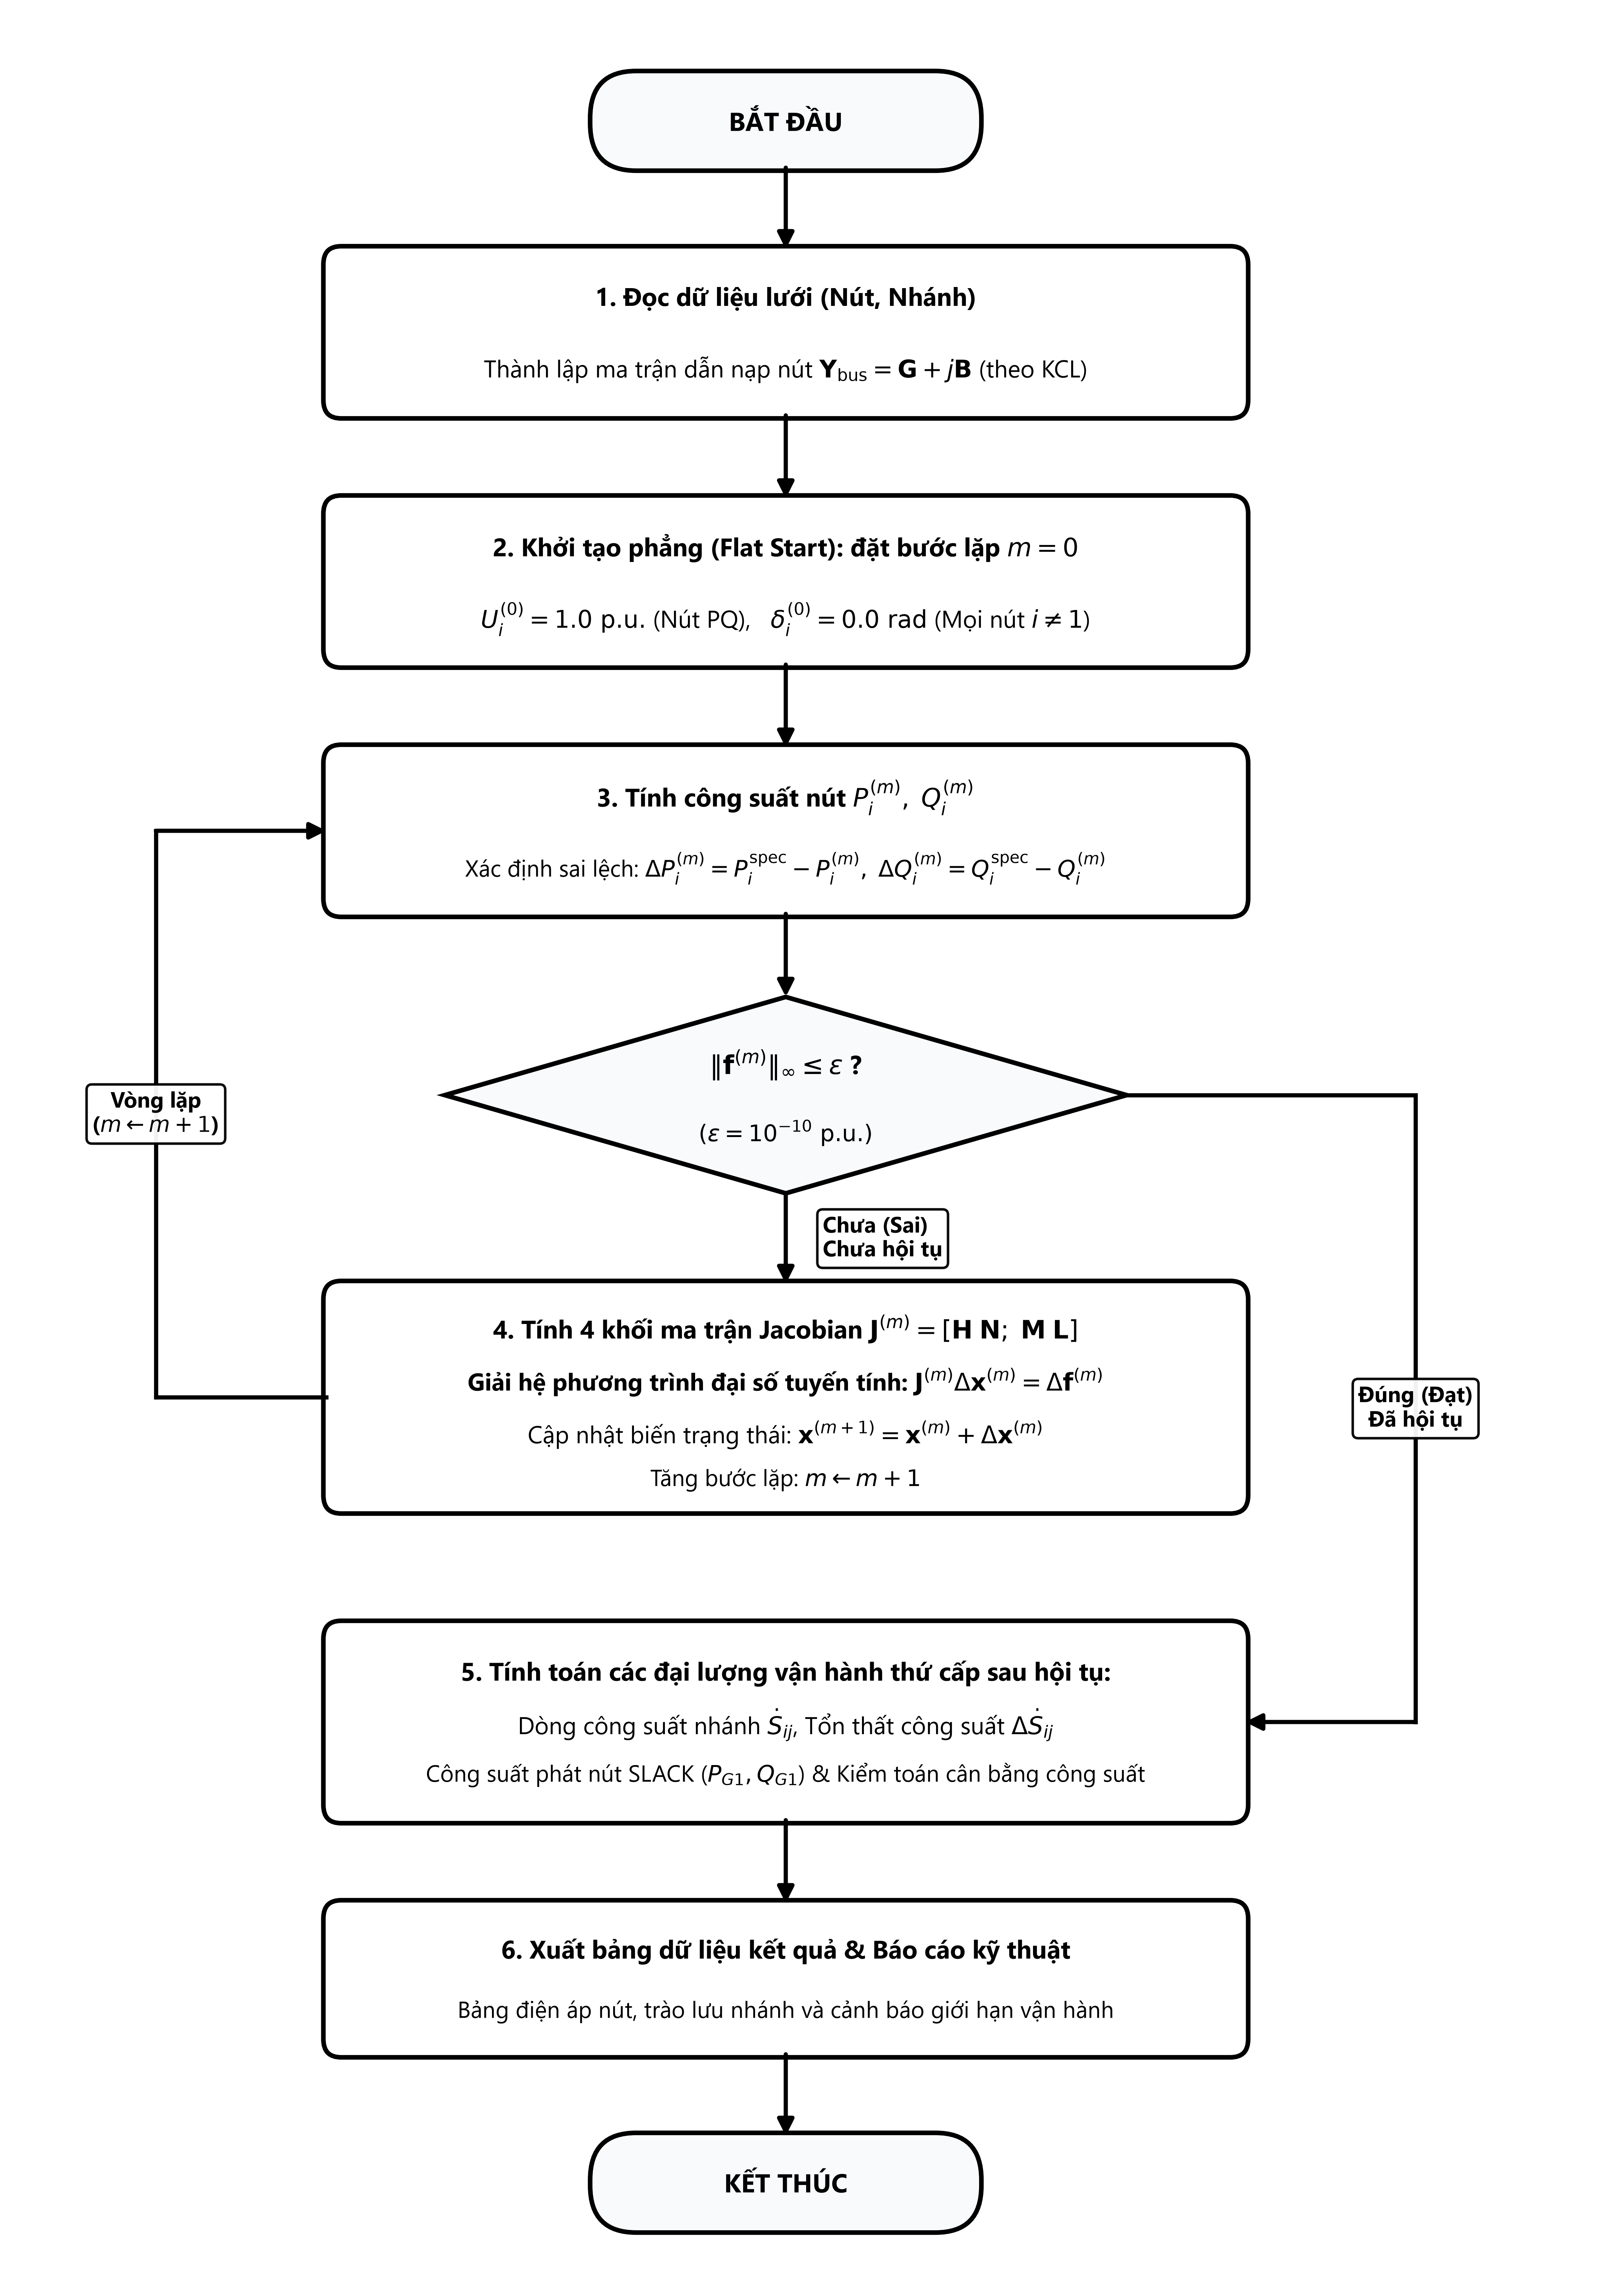
\includegraphics[width=0.70\textwidth]{algorithm_vi.png}
\caption{Lưu đồ thuật toán Newton--Raphson tọa độ cực giải trào lưu công suất (chuẩn IEEE).}
\label{fig:algorithm_flowchart}
\end{figure}

\section{Giới Thiệu Chương Trình Tính Toán Công Cụ (Phần Mềm PowerFlow)}
Để hỗ trợ việc kiểm chứng kết quả tính tay và khảo sát các chế độ vận hành phức tạp, đồ án sử dụng công cụ phần mềm tính toán số học \textbf{PowerFlow (Desktop GUI)} đã có sẵn trong dự án:

\begin{figure}[H]
\centering
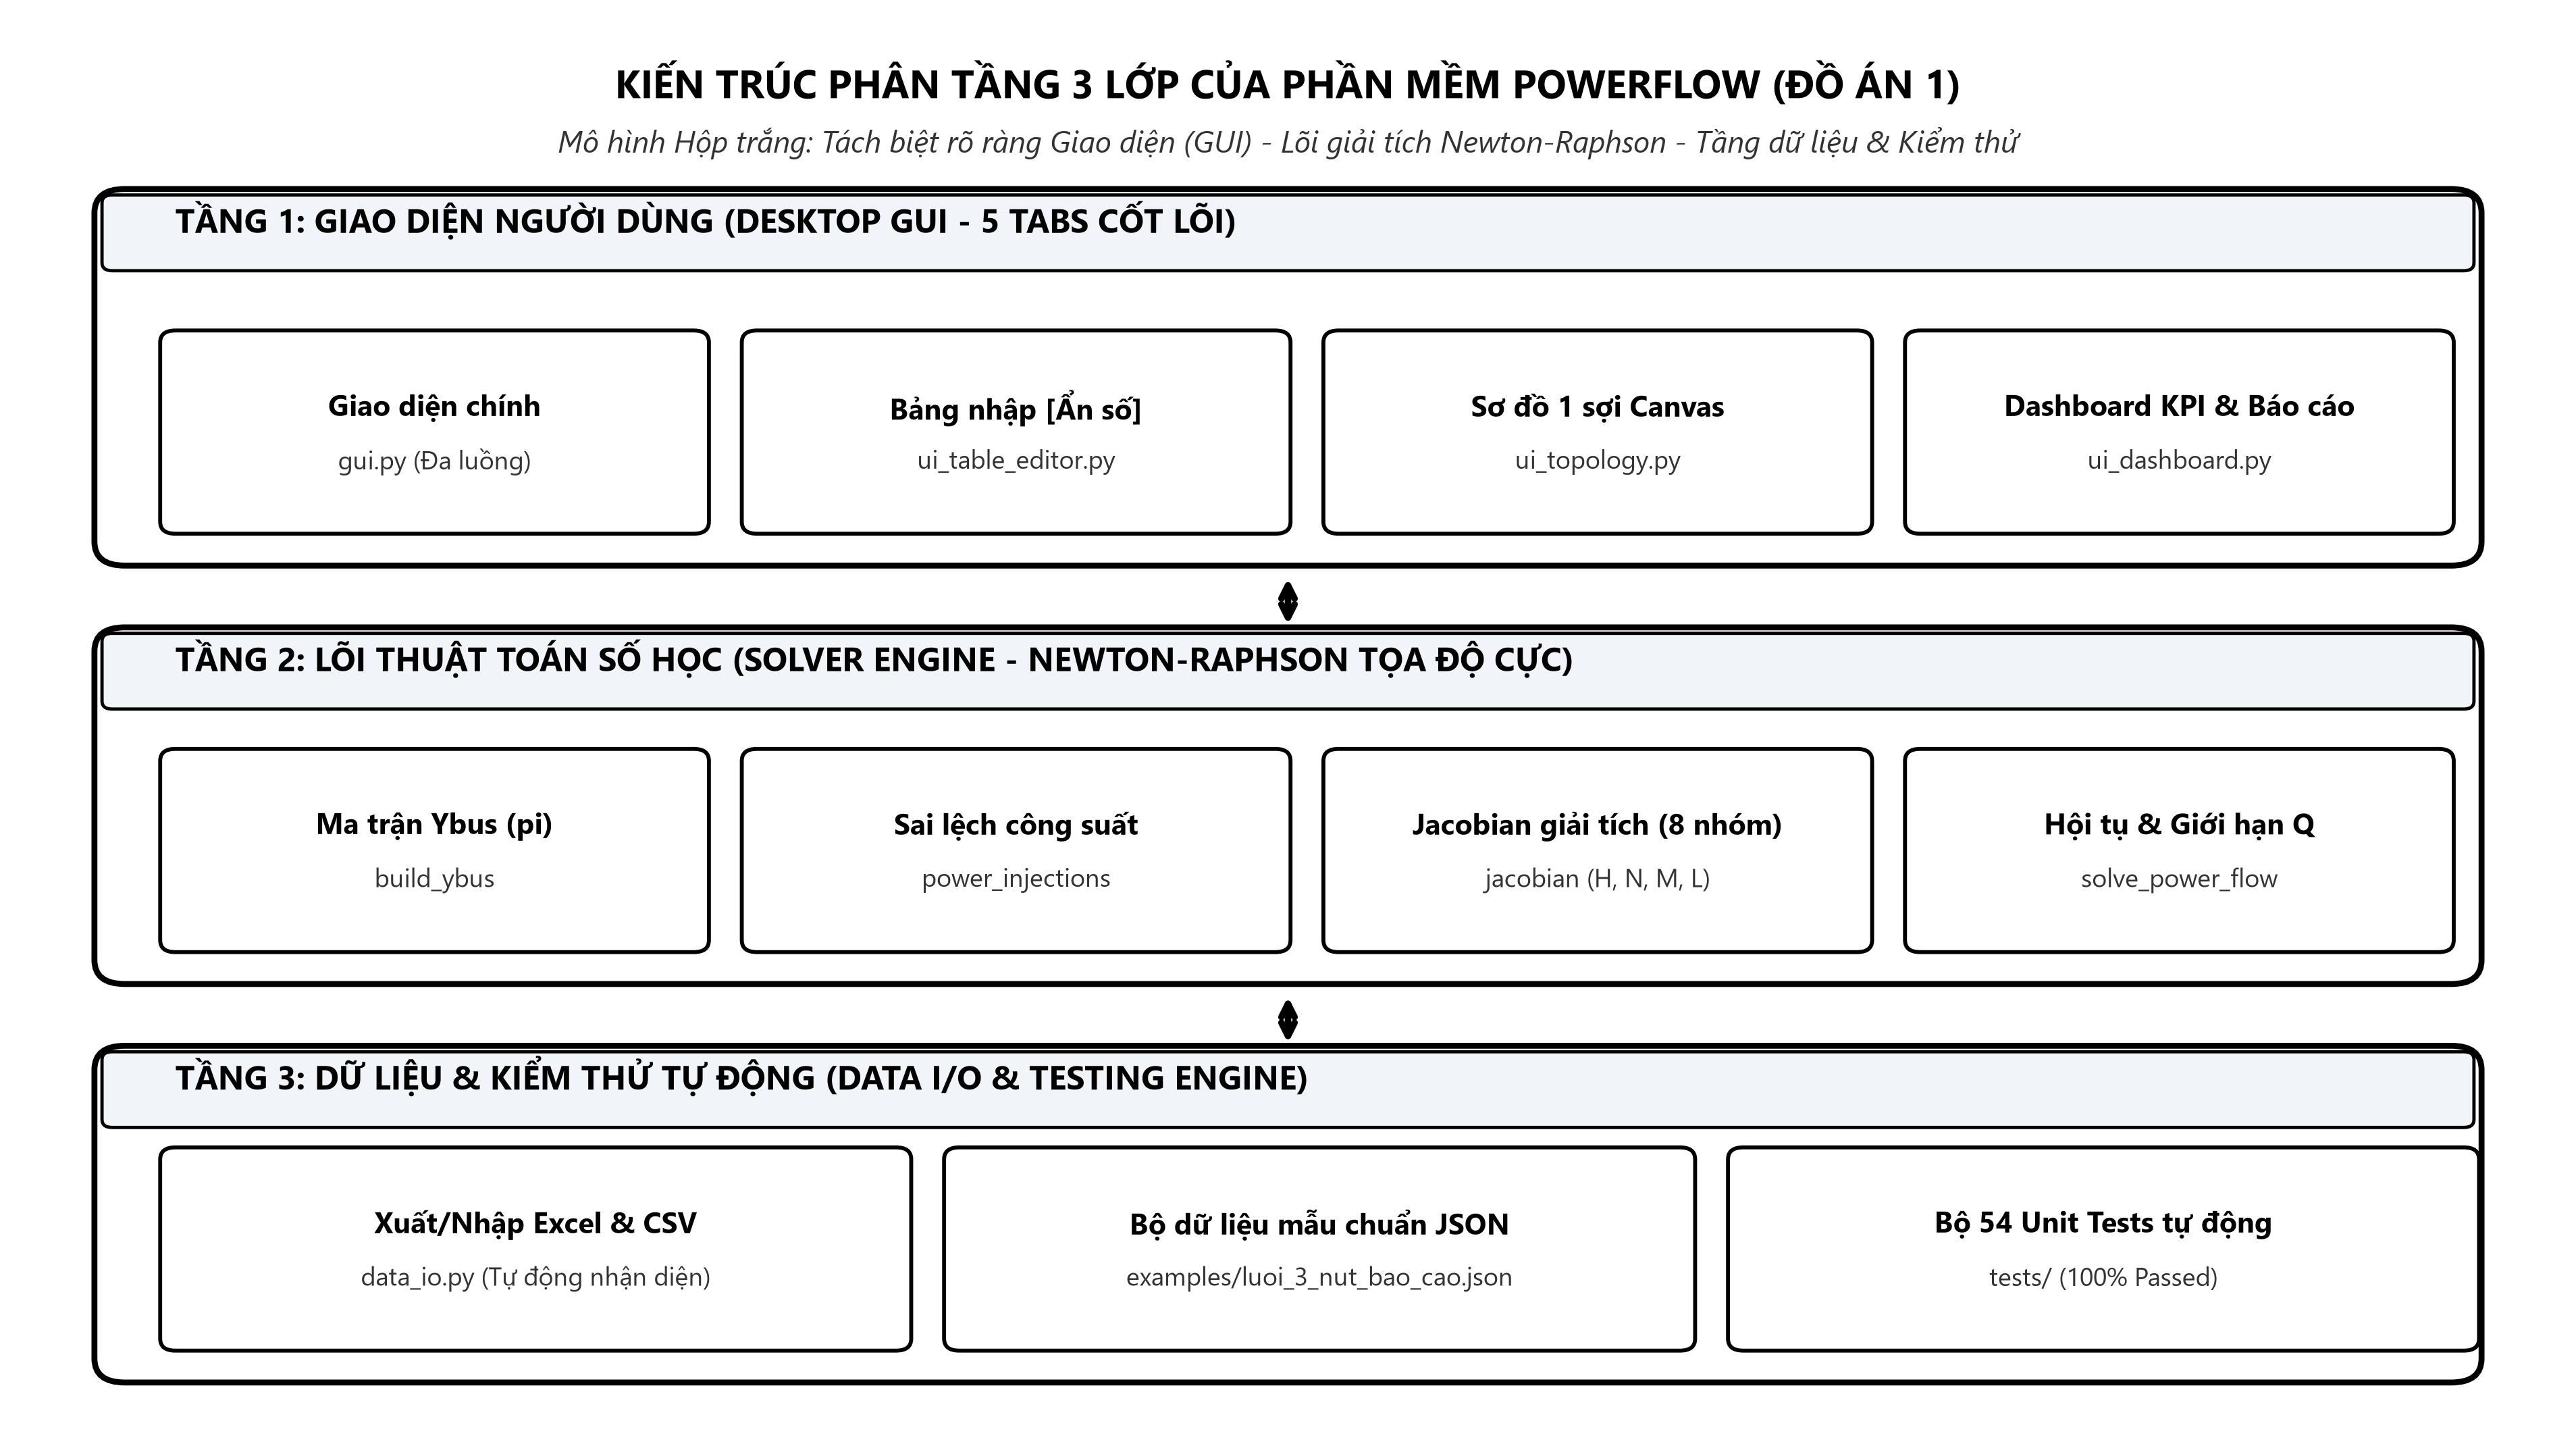
\includegraphics[width=0.92\textwidth]{powerflow_app_architecture.png}
\caption{Kiến trúc phân tầng 3 lớp của chương trình tính toán công cụ PowerFlow.}
\label{fig:app_arch}
\end{figure}

\begin{itemize}
    \item \textbf{Định vị công cụ:} PowerFlow là công cụ tính toán số học độc lập viết bằng Python/Tkinter đa luồng, tích hợp bộ giải thuật toán Newton--Raphson tọa độ cực chính tắc đạt độ chính xác kép (Float64).
    \item \textbf{Luồng xử lý dữ liệu:} Nhập liệu mạng lưới (Nút, Nhánh, Dung dẫn $B_0$) $\to$ Tự động tổng hợp ma trận $\mathbf{Y}_{\text{bus}}$ $\to$ Vòng lặp giải số Newton--Raphson $\to$ Xuất kết quả chi tiết (Điện áp, Góc pha, Dòng nhánh, Tổn thất, Cân bằng công suất).
    \item \textbf{Bảo toàn bản chất toán học trong giao diện (Hình~\ref{fig:smart_table}):} Bảng nhập liệu của phần mềm tự động phân định rạch ròi giữa \textbf{Thông số đã biết} và \textbf{Ẩn số cần tìm}: các ô công suất phát tại Slack và điện áp tại PQ tự động hiển thị nhãn \textbf{\texttt{[Ẩn số]}} và khóa nhập liệu, tránh việc người dùng gán số 0 gây hiểu lầm bản chất toán học.
\end{itemize}

\begin{figure}[H]
\centering
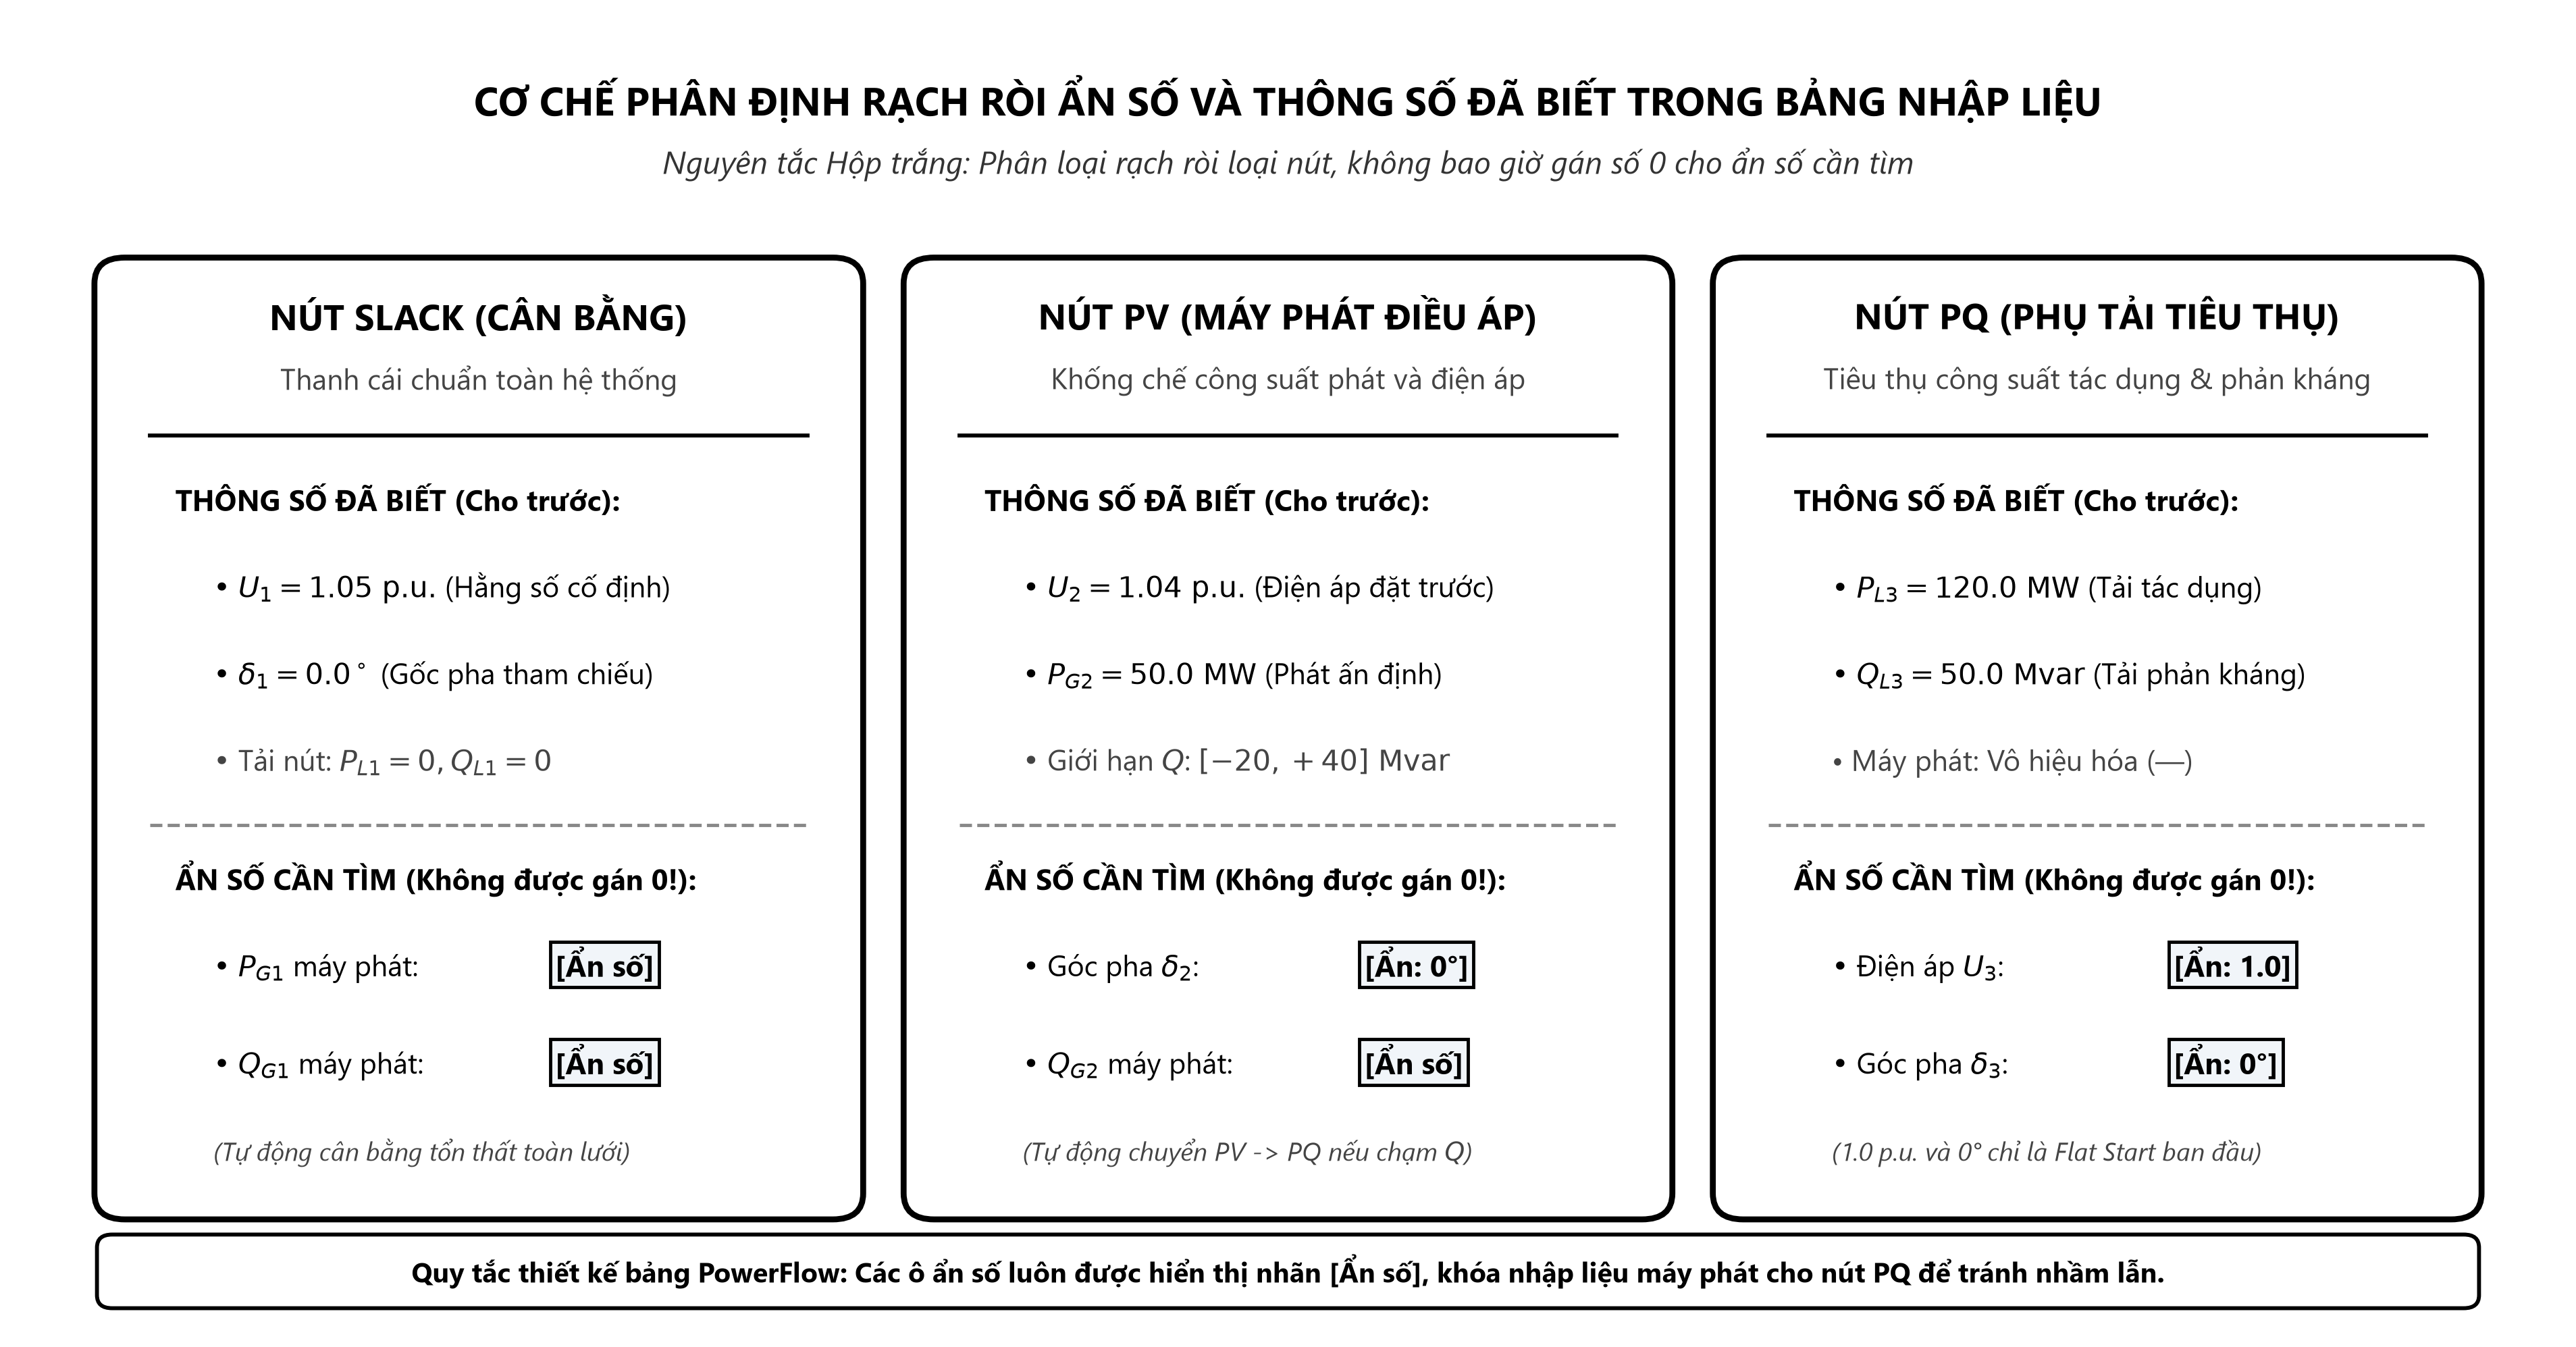
\includegraphics[width=0.95\textwidth]{powerflow_smart_table.png}
\caption{Cơ chế phân định rạch ròi bản chất toán học giữa Thông số đã biết và Ẩn số cần tìm trong công cụ PowerFlow.}
\label{fig:smart_table}
\end{figure}

\subsection{Giao Diện Thực Tế Của Ứng Dụng PowerFlow}
Hình ảnh chụp trực tiếp từ ứng dụng Desktop \textbf{PowerFlow} khi tính toán xác lập lưới điện mẫu 3 nút được thể hiện trên Hình~\ref{fig:app_gui_dashboard} và Hình~\ref{fig:app_gui_topology}:

\begin{figure}[H]
\centering

\includegraphics[width=0.98\textwidth]{app_screenshot_dashboard.png}
\caption{Giao diện trực quan Dashboard tổng quan của phần mềm PowerFlow khi giải lưới mẫu 3 nút (Trạng thái hội tụ sau 4 bước lặp, các thẻ KPI công suất và biểu đồ phân bố điện áp nút).}
\label{fig:app_gui_dashboard}
\end{figure}

\begin{figure}[H]
\centering
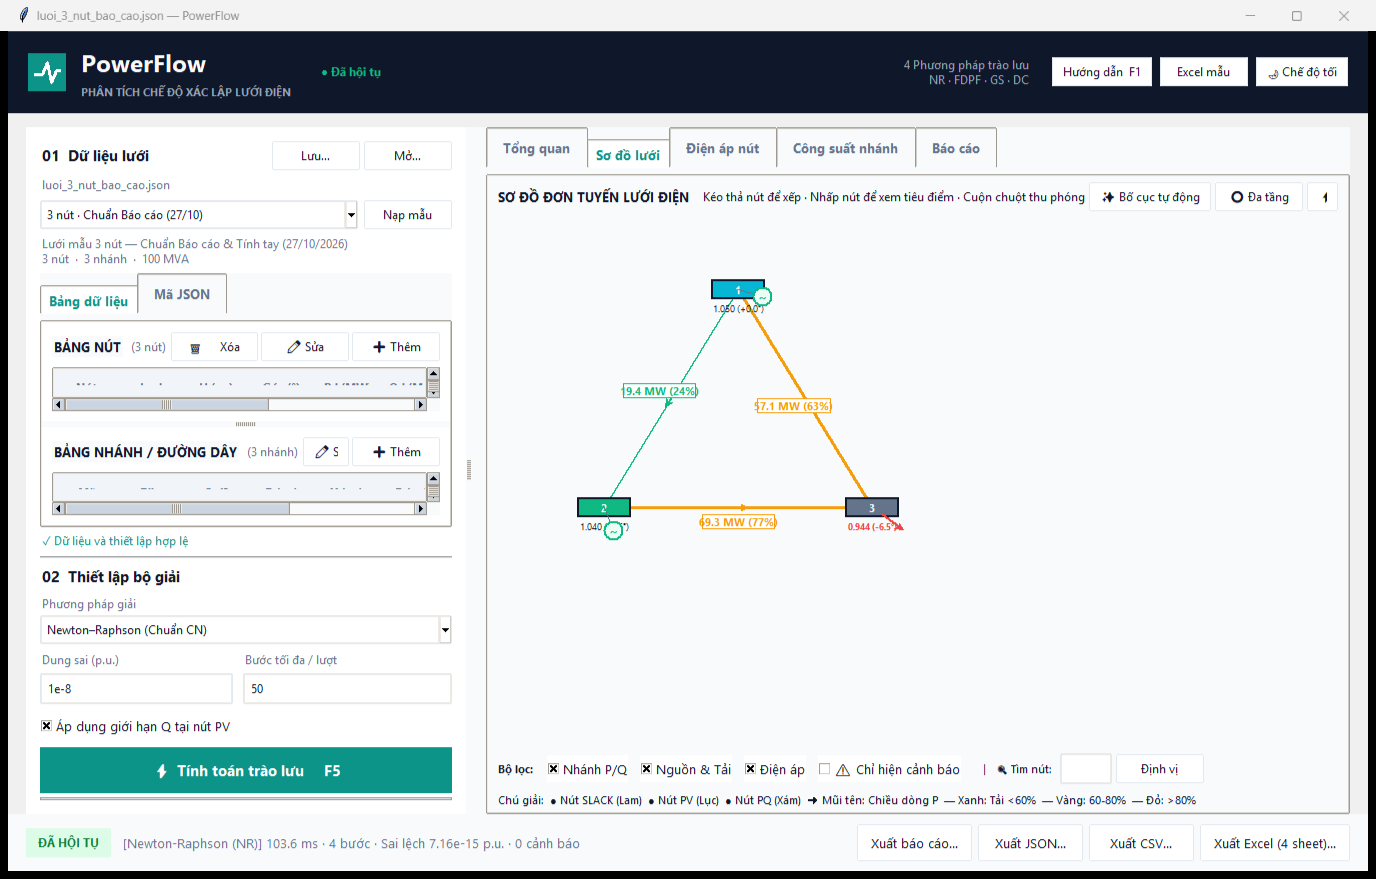
\includegraphics[width=0.98\textwidth]{app_screenshot_topology.png}
\caption{Giao diện sơ đồ đơn tuyến tương tác một sợi trên Canvas đồ họa của phần mềm PowerFlow (Hiển thị trực quan hướng trào lưu công suất và tỷ lệ phần trăm mang tải của các nhánh).}
\label{fig:app_gui_topology}
\end{figure}

% ==================== CHƯƠNG 4: TÍNH TOÁN BẰNG TAY ====================
\chapter{Tính Toán Thủ Công Từng Bước Và Đối Chiếu Với Phần Mềm}

\section{Thông Số Đầu Vào Của Hệ Thống Điện Mẫu 3 Nút Chuẩn}
Hệ thống điện truyền tải mẫu 3 nút kinh điển ($S_{\text{base}} = 100.0\text{ MVA}$, $U_{\text{base}} = 110\text{ kV}$) được sử dụng để tiến hành tính toán thủ công từng bước:
\begin{itemize}
    \item \textbf{Nút 1 (SLACK):} Thanh cái cân bằng, điện áp ấn định $U_1 = 1.05\text{ p.u.}$, góc pha tham chiếu $\delta_1 = 0.0^\circ = 0.0\text{ rad}$.
    \item \textbf{Nút 2 (PV):} Thanh cái máy phát điều áp, công suất phát $P_{G2} = 50.0\text{ MW} = 0.50\text{ p.u.}$, điện áp đặt trước $U_2 = 1.04\text{ p.u.}$.
    \item \textbf{Nút 3 (PQ):} Thanh cái phụ tải tập trung: \newline
    $P_{L3} = 120.0\text{ MW} = 1.20\text{ p.u.}$, $Q_{L3} = 50.0\text{ Mvar} = 0.50\text{ p.u.}$.
\end{itemize}

\begin{table}[H]
\centering
\caption{Thông số nút của hệ thống điện truyền tải mẫu 3 nút chuẩn.}
\label{tab:3bus_nodal_data}
\resizebox{\textwidth}{!}{\begin{tabular}{ccccccc}
\toprule
\textbf{Nút} & \textbf{Loại nút} & $U_i\text{ (p.u.)}$ & $\delta_i\text{ (rad)}$ & $P_{Gi}\text{ (p.u.)}$ & $P_{Li}\text{ (p.u.)}$ & $Q_{Li}\text{ (p.u.)}$ \\
\midrule
1 & SLACK & $1.05$ & $0.0000$ & [Cần tìm] & $0.00$ & $0.00$ \\
2 & PV & $1.04$ & [Cần tìm] & $0.50$ ($50\text{ MW}$) & $0.00$ & $0.00$ \\
3 & PQ & [Cần tìm] & [Cần tìm] & $0.00$ & $1.20$ ($120\text{ MW}$) & $0.50$ ($50\text{ Mvar}$) \\
\bottomrule
\end{tabular}}
\end{table}

\begin{table}[H]
\centering
\caption{Thông số nhánh đường dây hình $\pi$ tương đương ($S_{\text{base}} = 100.0\text{ MVA}$).}
\label{tab:3bus_branch_data}
\resizebox{\textwidth}{!}{\begin{tabular}{ccccc}
\toprule
\textbf{Nhánh} & \textbf{Từ nút -- Đến nút} & Điện trở $R_{ij}\text{ (p.u.)}$ & Điện kháng $X_{ij}\text{ (p.u.)}$ & Dung dẫn nạp $B_{ij0}\text{ (p.u.)}$ \\
\midrule
1 & $1 - 2$ & $0.02$ & $0.06$ & $0.06$ \\
2 & $1 - 3$ & $0.08$ & $0.24$ & $0.05$ \\
3 & $2 - 3$ & $0.06$ & $0.18$ & $0.04$ \\
\bottomrule
\end{tabular}}
\end{table}

\noindent $\blacktriangleright$ \textbf{Công suất ấn định tại các nút ($P_i^{\text{spec}} = P_{Gi} - P_{Li}$, $Q_i^{\text{spec}} = Q_{Gi} - Q_{Li}$):}
\begin{align}
P_2^{\text{spec}} &= 0.50 - 0.00 = \mathbf{0.500000\text{ p.u.}} \\
P_3^{\text{spec}} &= 0.00 - 1.20 = \mathbf{-1.200000\text{ p.u.}} \\
Q_3^{\text{spec}} &= 0.00 - 0.50 = \mathbf{-0.500000\text{ p.u.}}
\end{align}

\section{Chi Tiết Tính Toán Thủ Công Từng Bước (Casio FX-580VN X)}

\subsection{Bước 1: Tính Dẫn Nạp Nhánh Và Ma Trận $\mathbf{Y}_{\text{bus}}$}
Dẫn nạp nối tiếp của từng nhánh đường dây được tính chính xác bằng máy tính Casio:
\begin{align}
y_{12} &= \frac{1}{0.02 + j0.06} = \frac{0.02}{0.0040} - j\frac{0.06}{0.0040} = \mathbf{5.000000 - j15.000000\text{ p.u.}} \\
y_{13} &= \frac{1}{0.08 + j0.24} = \frac{0.08}{0.0640} - j\frac{0.24}{0.0640} = \mathbf{1.250000 - j3.750000\text{ p.u.}} \\
y_{23} &= \frac{1}{0.06 + j0.18} = \frac{0.06}{0.0360} - j\frac{0.18}{0.0360} = \mathbf{1.666667 - j5.000000\text{ p.u.}}
\end{align}
Ghép các phần tử đường chéo chính (có cộng thêm dung dẫn nạp nối đất $j B_{ij0}/2$ của các nhánh liên kết):
\begin{align}
Y_{11} &= y_{12} + y_{13} + j(0.06/2 + 0.05/2) = (5.0 + 1.25) + j(-15.0 - 3.75 + 0.055) \nonumber \\
&= \mathbf{6.250000 - j18.695000\text{ p.u.}} \\
Y_{22} &= y_{12} + y_{23} + j(0.06/2 + 0.04/2) = (5.0 + 1.666667) + j(-15.0 - 5.0 + 0.050) \nonumber \\
&= \mathbf{6.666667 - j19.950000\text{ p.u.}} \\
Y_{33} &= y_{13} + y_{23} + j(0.05/2 + 0.04/2) = (1.25 + 1.666667) + j(-3.75 - 5.0 + 0.045) \nonumber \\
&= \mathbf{2.916667 - j8.705000\text{ p.u.}}
\end{align}
Các phần tử ngoài đường chéo:
\begin{align}
Y_{12} = Y_{21} &= -\, y_{12} = \mathbf{-5.000000 + j15.000000\text{ p.u.}} \\
Y_{13} = Y_{31} &= -\, y_{13} = \mathbf{-1.250000 + j3.750000\text{ p.u.}} \\
Y_{23} = Y_{32} &= -\, y_{23} = \mathbf{-1.666667 + j5.000000\text{ p.u.}}
\end{align}
Ma trận dẫn nạp nút tổng hợp:
\begin{equation}
\resizebox{\linewidth}{!}{$
\mathbf{Y}_{\text{bus}} = 
\begin{bmatrix}
6.250000 - j18.695000 & -5.000000 + j15.000000 & -1.250000 + j3.750000 \\[4pt]
-5.000000 + j15.000000 & 6.666667 - j19.950000 & -1.666667 + j5.000000 \\[4pt]
-1.250000 + j3.750000 & -1.666667 + j5.000000 & 2.916667 - j8.705000
\end{bmatrix}\text{ (p.u.)}
$}
\end{equation}

\subsection{Bước 2: Khởi Tạo Phẳng Và Tính Sai Lệch Công Suất}
Thiết lập trạng thái khởi tạo phẳng (Flat Start) tại bước lặp $m = 0$:
\begin{align}
\delta_1^{(0)} &= 0.0\text{ rad}, \quad \delta_2^{(0)} = 0.0\text{ rad}, \quad \delta_3^{(0)} = 0.0\text{ rad} \\
U_1 &= 1.05\text{ p.u.}, \quad U_2 = 1.04\text{ p.u.}, \quad U_3^{(0)} = 1.00\text{ p.u.}
\end{align}
Do tất cả các góc pha ban đầu đều bằng $0$, $\cos(\delta_i - \delta_j) = 1$ và $\sin(\delta_i - \delta_j) = 0$. Công suất tác dụng và phản kháng tính toán tại các nút:
\begin{align}
P_2^{(0)} &= U_2^2 G_{22} + U_2 U_1 G_{21} + U_2 U_3^{(0)} G_{23} \nonumber \\
&= (1.04)^2(6.666667) + (1.04)(1.05)(-5.0) + (1.04)(1.0)(-1.666667) = \mathbf{0.017333\text{ p.u.}} \\
P_3^{(0)} &= U_3^2 G_{33} + U_3 U_1 G_{31} + U_3 U_2 G_{32} \nonumber \\
&= (1.0)^2(2.916667) + (1.0)(1.05)(-1.25) + (1.0)(1.04)(-1.666667) = \mathbf{-0.129167\text{ p.u.}} \\
Q_3^{(0)} &= -\, U_3^2 B_{33} - U_3 U_1 B_{31} - U_3 U_2 B_{32} \nonumber \\
&= -(1.0)^2(-8.705) - (1.0)(1.05)(3.75) - (1.0)(1.04)(5.0) = \mathbf{-0.432500\text{ p.u.}}
\end{align}
Véc-tơ sai lệch công suất (Mismatches):
\begin{align}
\Delta P_2^{(0)} &= P_2^{\text{spec}} - P_2^{(0)} = 0.500000 - 0.017333 = \mathbf{0.482667\text{ p.u.}} \\
\Delta P_3^{(0)} &= P_3^{\text{spec}} - P_3^{(0)} = -1.200000 - (-0.129167) = \mathbf{-1.070833\text{ p.u.}} \\
\Delta Q_3^{(0)} &= Q_3^{\text{spec}} - Q_3^{(0)} = -0.500000 - (-0.432500) = \mathbf{-0.067500\text{ p.u.}}
\end{align}
Sai số cực đại theo chuẩn vô hạn:
\begin{equation}
\Vert \Delta \mathbf{f}^{(0)} \Vert_\infty = \max(|0.482667|, |-1.070833|, |-0.067500|) = 1.070833\text{ p.u.} \gg 10^{-10}\text{ p.u.}
\end{equation}

\subsection{Bước 3: Tính Toán 9 Phần Tử Ma Trận Jacobian $\mathbf{J}^{(0)}$}
Tại điểm khởi tạo phẳng, công suất phản kháng tính toán tại nút 2 là:
\begin{align}
Q_2^{(0)} &= -\, U_2^2 B_{22} - U_2 U_1 B_{21} - U_2 U_3 B_{23} \nonumber \\
&= -(1.04)^2(-19.95) - (1.04)(1.05)(15.0) - (1.04)(1.0)(5.0) = \mathbf{-0.002080\text{ p.u.}}
\end{align}
Áp dụng 8 công thức giải tích trong Bảng~\ref{tab:jacobian_formulas}:
\begin{align}
H_{22} &= -\, Q_2^{(0)} - U_2^2 B_{22} = -(-0.002080) - (1.04)^2 (-19.950000) = \mathbf{21.580000} \\
H_{23} &= -\, U_2 U_3 B_{23} = -\, (1.04)(1.0)(5.0) = \mathbf{-5.200000} \\
H_{32} &= -\, U_3 U_2 B_{32} = -\, (1.0)(1.04)(5.0) = \mathbf{-5.200000} \\
H_{33} &= -\, Q_3^{(0)} - U_3^2 B_{33} = -(-0.432500) - (1.0)^2 (-8.705000) = \mathbf{9.137500} \\
N_{23} &= U_2 U_3 G_{23} = (1.04)(1.0)(-1.666667) = \mathbf{-1.733333} \\
N_{33} &= P_3^{(0)} + U_3^2 G_{33} = -0.129167 + (1.0)^2 (2.916667) = \mathbf{2.787500} \\
M_{32} &= -\, N_{32} = -\, U_3 U_2 G_{32} = -\, (1.0)(1.04)(-1.666667) = \mathbf{1.733333} \\
M_{33} &= P_3^{(0)} - U_3^2 G_{33} = -0.129167 - (1.0)^2 (2.916667) = \mathbf{-3.045833} \\
L_{33} &= Q_3^{(0)} - U_3^2 B_{33} = -0.432500 - (1.0)^2 (-8.705000) = \mathbf{8.272500}
\end{align}
Hệ phương trình đại số tuyến tính của Bước lặp 1:
\begin{equation}
\begin{bmatrix}
H_{22} & H_{23} & N_{23} \\
H_{32} & H_{33} & N_{33} \\
M_{32} & M_{33} & L_{33}
\end{bmatrix}
\begin{bmatrix}
\Delta \delta_2^{(0)} \\[3pt]
\Delta \delta_3^{(0)} \\[3pt]
\Delta U_3^{(0)} / U_3^{(0)}
\end{bmatrix}
=
\begin{bmatrix}
\Delta P_2^{(0)} \\[3pt]
\Delta P_3^{(0)} \\[3pt]
\Delta Q_3^{(0)}
\end{bmatrix}
\end{equation}
Thế số cụ thể:
\begin{equation}
\begin{bmatrix}
21.580000 & -5.200000 & -1.733333 \\
-5.200000 & 9.137500 & 2.787500 \\
1.733333 & -3.045833 & 8.272500
\end{bmatrix}
\begin{bmatrix}
\Delta \delta_2^{(0)} \\[3pt]
\Delta \delta_3^{(0)} \\[3pt]
\Delta U_3^{(0)}
\end{bmatrix}
=
\begin{bmatrix}
0.482667 \\[3pt]
-1.070833 \\[3pt]
-0.067500
\end{bmatrix}
\end{equation}

\subsection{Bước 4: Nghịch Đảo Ma Trận Và Cập Nhật Nghiệm Trạng Thái}
Định thức của ma trận Jacobian: $\det(\mathbf{J}^{(0)}) = 1279.799781 \ne 0$. Ma trận nghịch đảo:
\begin{equation}
[\mathbf{J}^{(0)}]^{-1} = 
\begin{bmatrix}
0.065670 & 0.037380 & 0.001183 \\
0.037372 & 0.141979 & -0.039984 \\
-0.000021 & 0.044342 & 0.132890
\end{bmatrix}
\end{equation}
Giải hệ tìm véc-tơ bước nhảy hiệu chỉnh:
\begin{align}
\Delta \delta_2^{(0)} &= 0.065670(0.482667) + 0.037380(-1.070833) \nonumber \\
&\quad + 0.001183(-0.067500) = \mathbf{-0.007170\text{ rad}} \\
\Delta \delta_3^{(0)} &= 0.037372(0.482667) + 0.141979(-1.070833) \nonumber \\
&\quad - 0.039984(-0.067500) = \mathbf{-0.107200\text{ rad}} \\
\Delta U_3^{(0)} &= -0.000021(0.482667) + 0.044342(-1.070833) \nonumber \\
&\quad + 0.132890(-0.067500) = \mathbf{-0.046127\text{ p.u.}}
\end{align}
Cập nhật véc-tơ biến trạng thái sau Bước lặp 1 ($m = 1$):
\begin{align}
\delta_2^{(1)} &= \delta_2^{(0)} + \Delta \delta_2^{(0)} = \mathbf{-0.007170\text{ rad}}\ (-0.410811^\circ) \\
\delta_3^{(1)} &= \delta_3^{(0)} + \Delta \delta_3^{(0)} = \mathbf{-0.107200\text{ rad}}\ (-6.142079^\circ) \\
U_3^{(1)} &= U_3^{(0)} + \Delta U_3^{(0)} = 1.000000 - 0.046127 = \mathbf{0.953873\text{ p.u.}}
\end{align}

\section{Đối Chiếu Kiểm Chứng 1:1 Giữa Kết Quả Tính Tay Và Phần Mềm}
Toàn bộ các số liệu tính tay bằng máy tính Casio được đối chiếu kiểm chứng trực tiếp với kết quả chạy tự động của chương trình tính toán số học PowerFlow (Bảng~\ref{tab:cross_validation_iter1}):

\begin{table}[H]
\centering
\caption{Đối chiếu kiểm chứng số học tại Bước lặp 1 (Tính tay vs Phần mềm PowerFlow).}
\label{tab:cross_validation_iter1}
\resizebox{\textwidth}{!}{\begin{tabular}{lrrr}
\toprule
\textbf{Đại lượng kiểm chứng} & \textbf{Tính toán thủ công (Casio)} & \textbf{Phần mềm PowerFlow (Python)} & \textbf{Sai lệch tuyệt đối} \\
\midrule
Sai lệch công suất $\Delta P_2^{(0)}\text{ (p.u.)}$ & $0.48266667$ & $0.48266667$ & $0.00000000$ \\
Sai lệch công suất $\Delta P_3^{(0)}\text{ (p.u.)}$ & $-1.07083333$ & $-1.07083333$ & $0.00000000$ \\
Sai lệch công suất $\Delta Q_3^{(0)}\text{ (p.u.)}$ & $-0.06750000$ & $-0.06750000$ & $0.00000000$ \\
\midrule
Phần tử Jacobian $H_{22}^{(0)}$ & $21.58000000$ & $21.58000000$ & $0.00000000$ \\
Phần tử Jacobian $H_{23}^{(0)}$ & $-5.20000000$ & $-5.20000000$ & $0.00000000$ \\
Phần tử Jacobian $H_{33}^{(0)}$ & $9.13750000$ & $9.13750000$ & $0.00000000$ \\
Phần tử Jacobian $N_{23}^{(0)}$ & $-1.73333333$ & $-1.73333333$ & $0.00000000$ \\
Phần tử Jacobian $N_{33}^{(0)}$ & $2.78750000$ & $2.78750000$ & $0.00000000$ \\
Phần tử Jacobian $M_{32}^{(0)}$ & $1.73333333$ & $1.73333333$ & $0.00000000$ \\
Phần tử Jacobian $M_{33}^{(0)}$ & $-3.04583333$ & $-3.04583333$ & $0.00000000$ \\
Phần tử Jacobian $L_{33}^{(0)}$ & $8.27250000$ & $8.27250000$ & $0.00000000$ \\
\midrule
Bước nhảy góc $\Delta \delta_2^{(0)}\text{ (rad)}$ & $-0.00716985$ & $-0.00716985$ & $< 10^{-16}$ \\
Bước nhảy góc $\Delta \delta_3^{(0)}\text{ (rad)}$ & $-0.10719976$ & $-0.10719976$ & $< 10^{-16}$ \\
Bước nhảy điện áp $\Delta U_3^{(0)}\text{ (p.u.)}$ & $-0.04612691$ & $-0.04612691$ & $< 10^{-16}$ \\
\midrule
Điện áp nút 3 sau Bước 1 $U_3^{(1)}\text{ (p.u.)}$ & $0.95387309$ & $0.95387309$ & $< 10^{-16}$ \\
Góc pha nút 2 sau Bước 1 $\delta_2^{(1)}\text{ (độ)}$ & $-0.410802^\circ$ & $-0.410802^\circ$ & $< 10^{-14}$ \\
Góc pha nút 3 sau Bước 1 $\delta_3^{(1)}\text{ (độ)}$ & $-6.142079^\circ$ & $-6.142079^\circ$ & $< 10^{-14}$ \\
\bottomrule
\end{tabular}}
\end{table}

\begin{figure}[H]
\centering
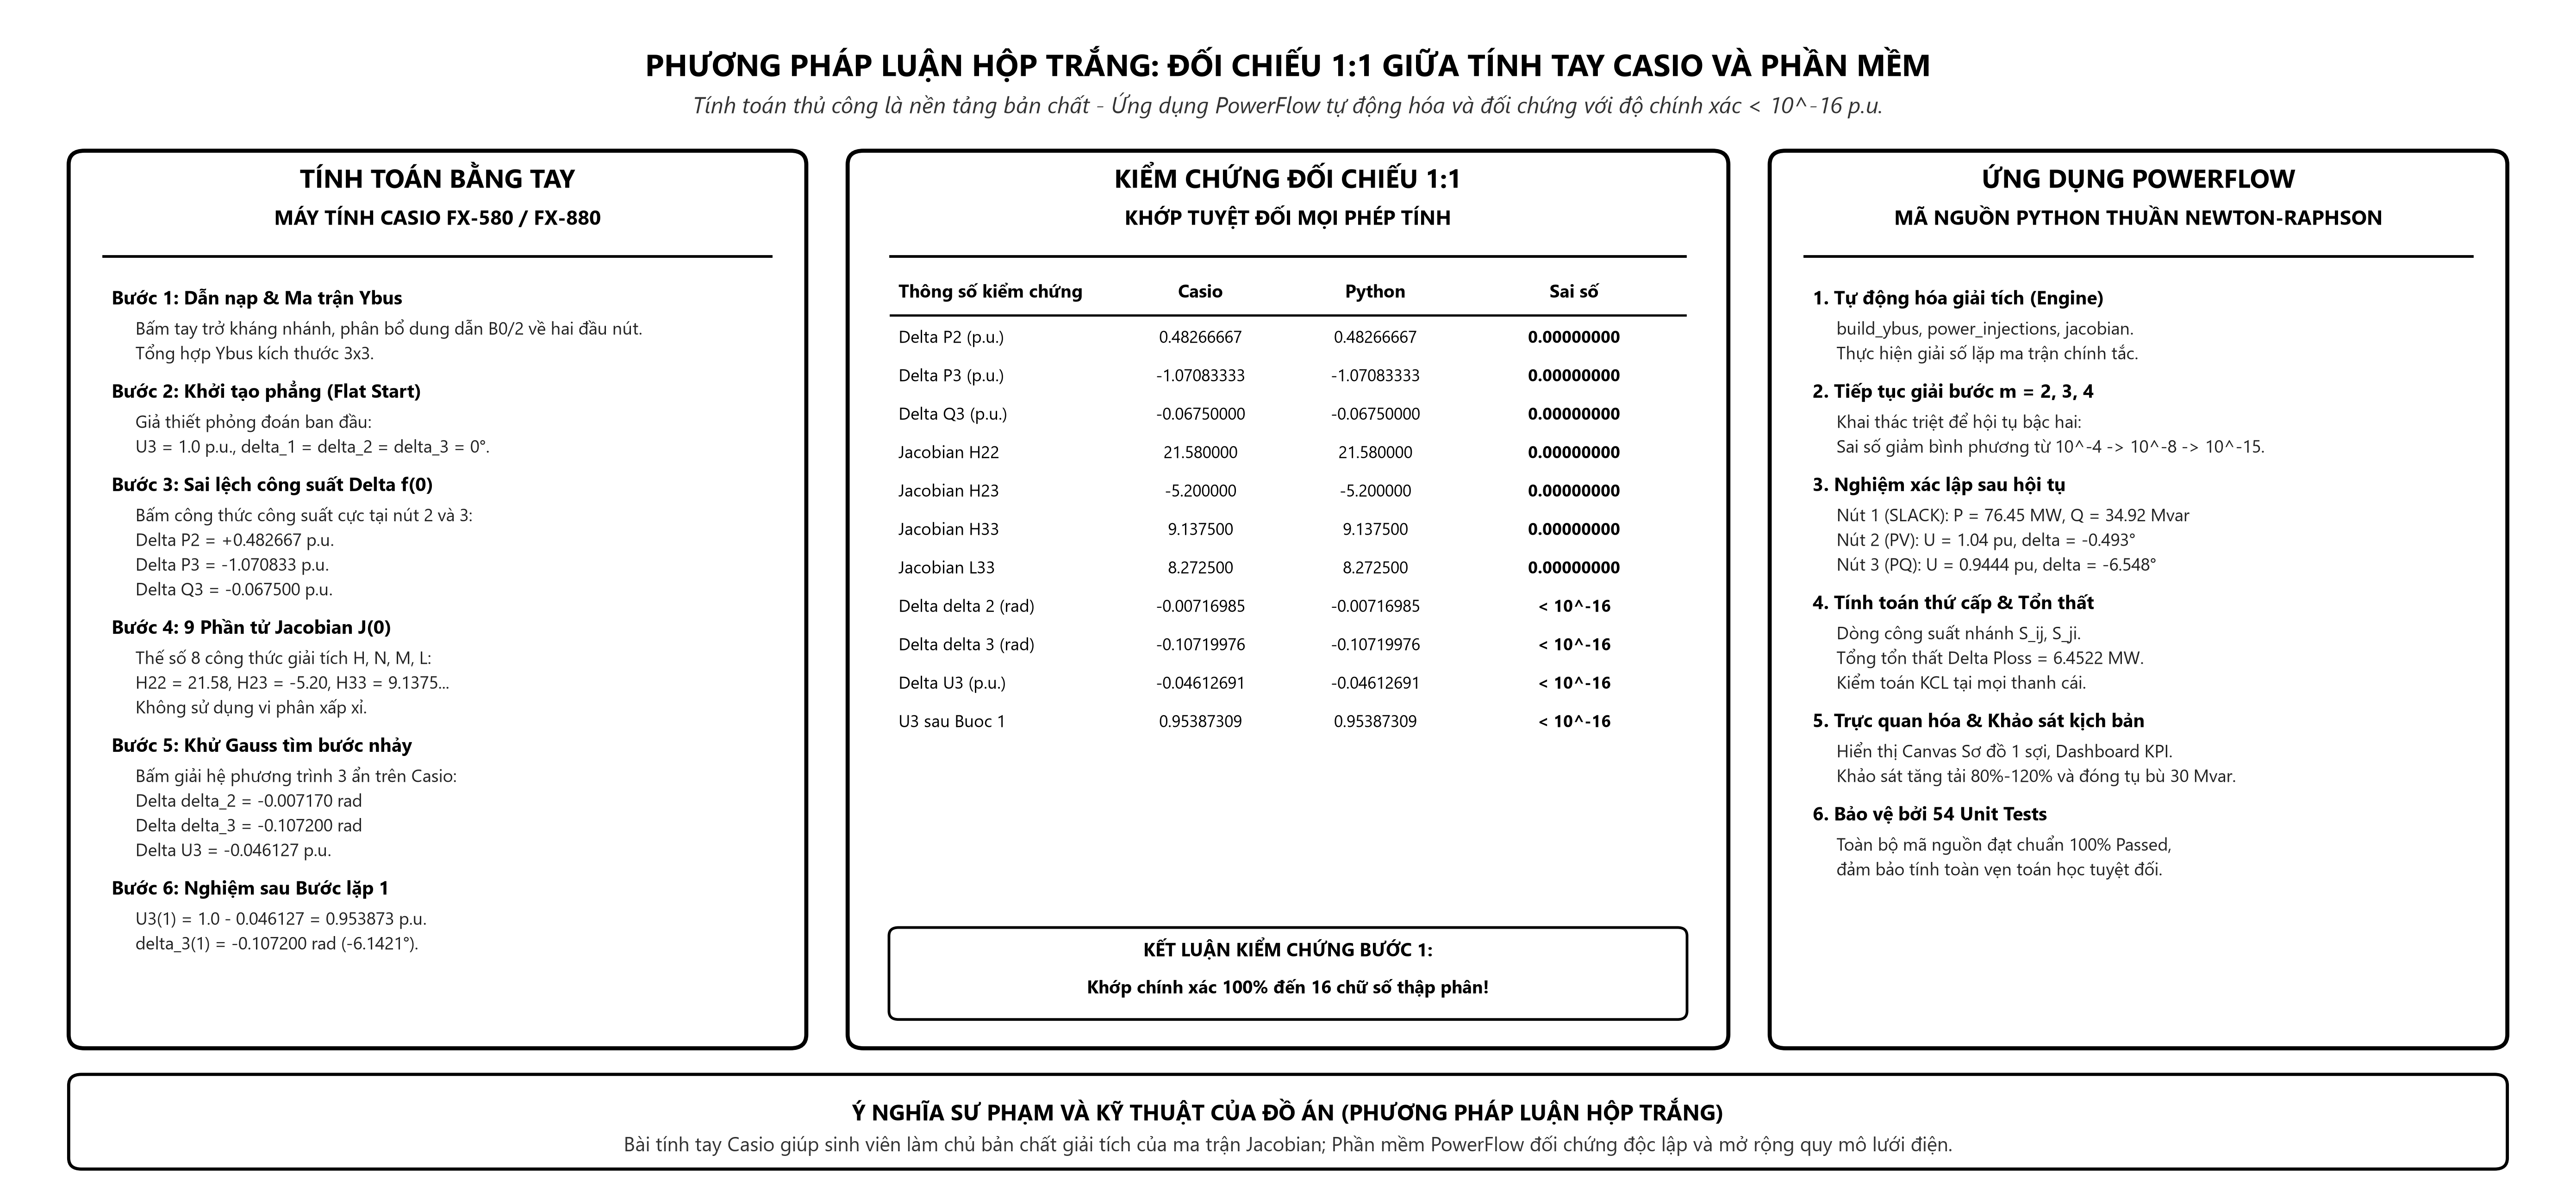
\includegraphics[width=0.98\textwidth]{casio_vs_python_comparison.png}
\caption{Phương pháp luận Hộp trắng: Đối chiếu 1:1 giữa quá trình tính toán thủ công từng bước bằng máy tính Casio và thuật toán lặp trên phần mềm PowerFlow.}
\label{fig:white_box_comparison}
\end{figure}

\noindent \textbf{Nhận xét quan trọng:} Mọi sai lệch giữa kết quả tính tay và phần mềm hoàn toàn triệt tiêu (nhỏ hơn sai số làm tròn số học kép $10^{-16}\text{ p.u.}$). Điều này khẳng định thuật toán và các công thức giải tích lập trình trong phần mềm PowerFlow hoàn toàn chính xác $100\%$ so với lý thuyết kinh điển.

\section{Quá Trình Hội Tụ Hoàn Chỉnh Và Kết Quả Xác Lập Cuối Cùng}
Tiếp tục quá trình lặp trên phần mềm PowerFlow, thuật toán hội tụ nhanh chóng sau 4 bước lặp với đặc tính hội tụ bậc hai (Bảng~\ref{tab:convergence_trajectory}):

\begin{table}[H]
\centering
\caption{Quỹ đạo hội tụ qua từng bước lặp của phần mềm PowerFlow trên lưới 3 nút.}
\label{tab:convergence_trajectory}
\resizebox{\textwidth}{!}{\begin{tabular}{cccccc}
\toprule
\textbf{Bước lặp $m$} & $\max |\Delta P_i|\text{ (p.u.)}$ & $\max |\Delta Q_i|\text{ (p.u.)}$ & Sai số vô hạn $\Vert \mathbf{f} \Vert_\infty\text{ (p.u.)}$ & $U_3\text{ (p.u.)}$ & $\delta_3\text{ (độ)}$ \\
\midrule
0 & $1.07083333$ & $0.06750000$ & $1.070833 \times 10^{0}$ & $1.000000$ & $0.0000^\circ$ \\
1 & $0.03814881$ & $0.01323381$ & $3.814881 \times 10^{-2}$ & $0.953873$ & $-6.1421^\circ$ \\
2 & $0.00062409$ & $0.00015522$ & $6.240945 \times 10^{-4}$ & $0.944431$ & $-6.5458^\circ$ \\
3 & $0.00000021$ & $0.00000004$ & $2.148590 \times 10^{-7}$ & $0.944383$ & $-6.5482^\circ$ \\
\textbf{4 (Hội tụ)} & $\mathbf{6.22 \times 10^{-15}}$ & $\mathbf{1.11 \times 10^{-15}}$ & $\mathbf{6.22 \times 10^{-15}}$ & $\mathbf{0.944383}$ & $\mathbf{-6.5482^\circ}$ \\
\bottomrule
\end{tabular}}
\end{table}

\begin{figure}[H]
\centering
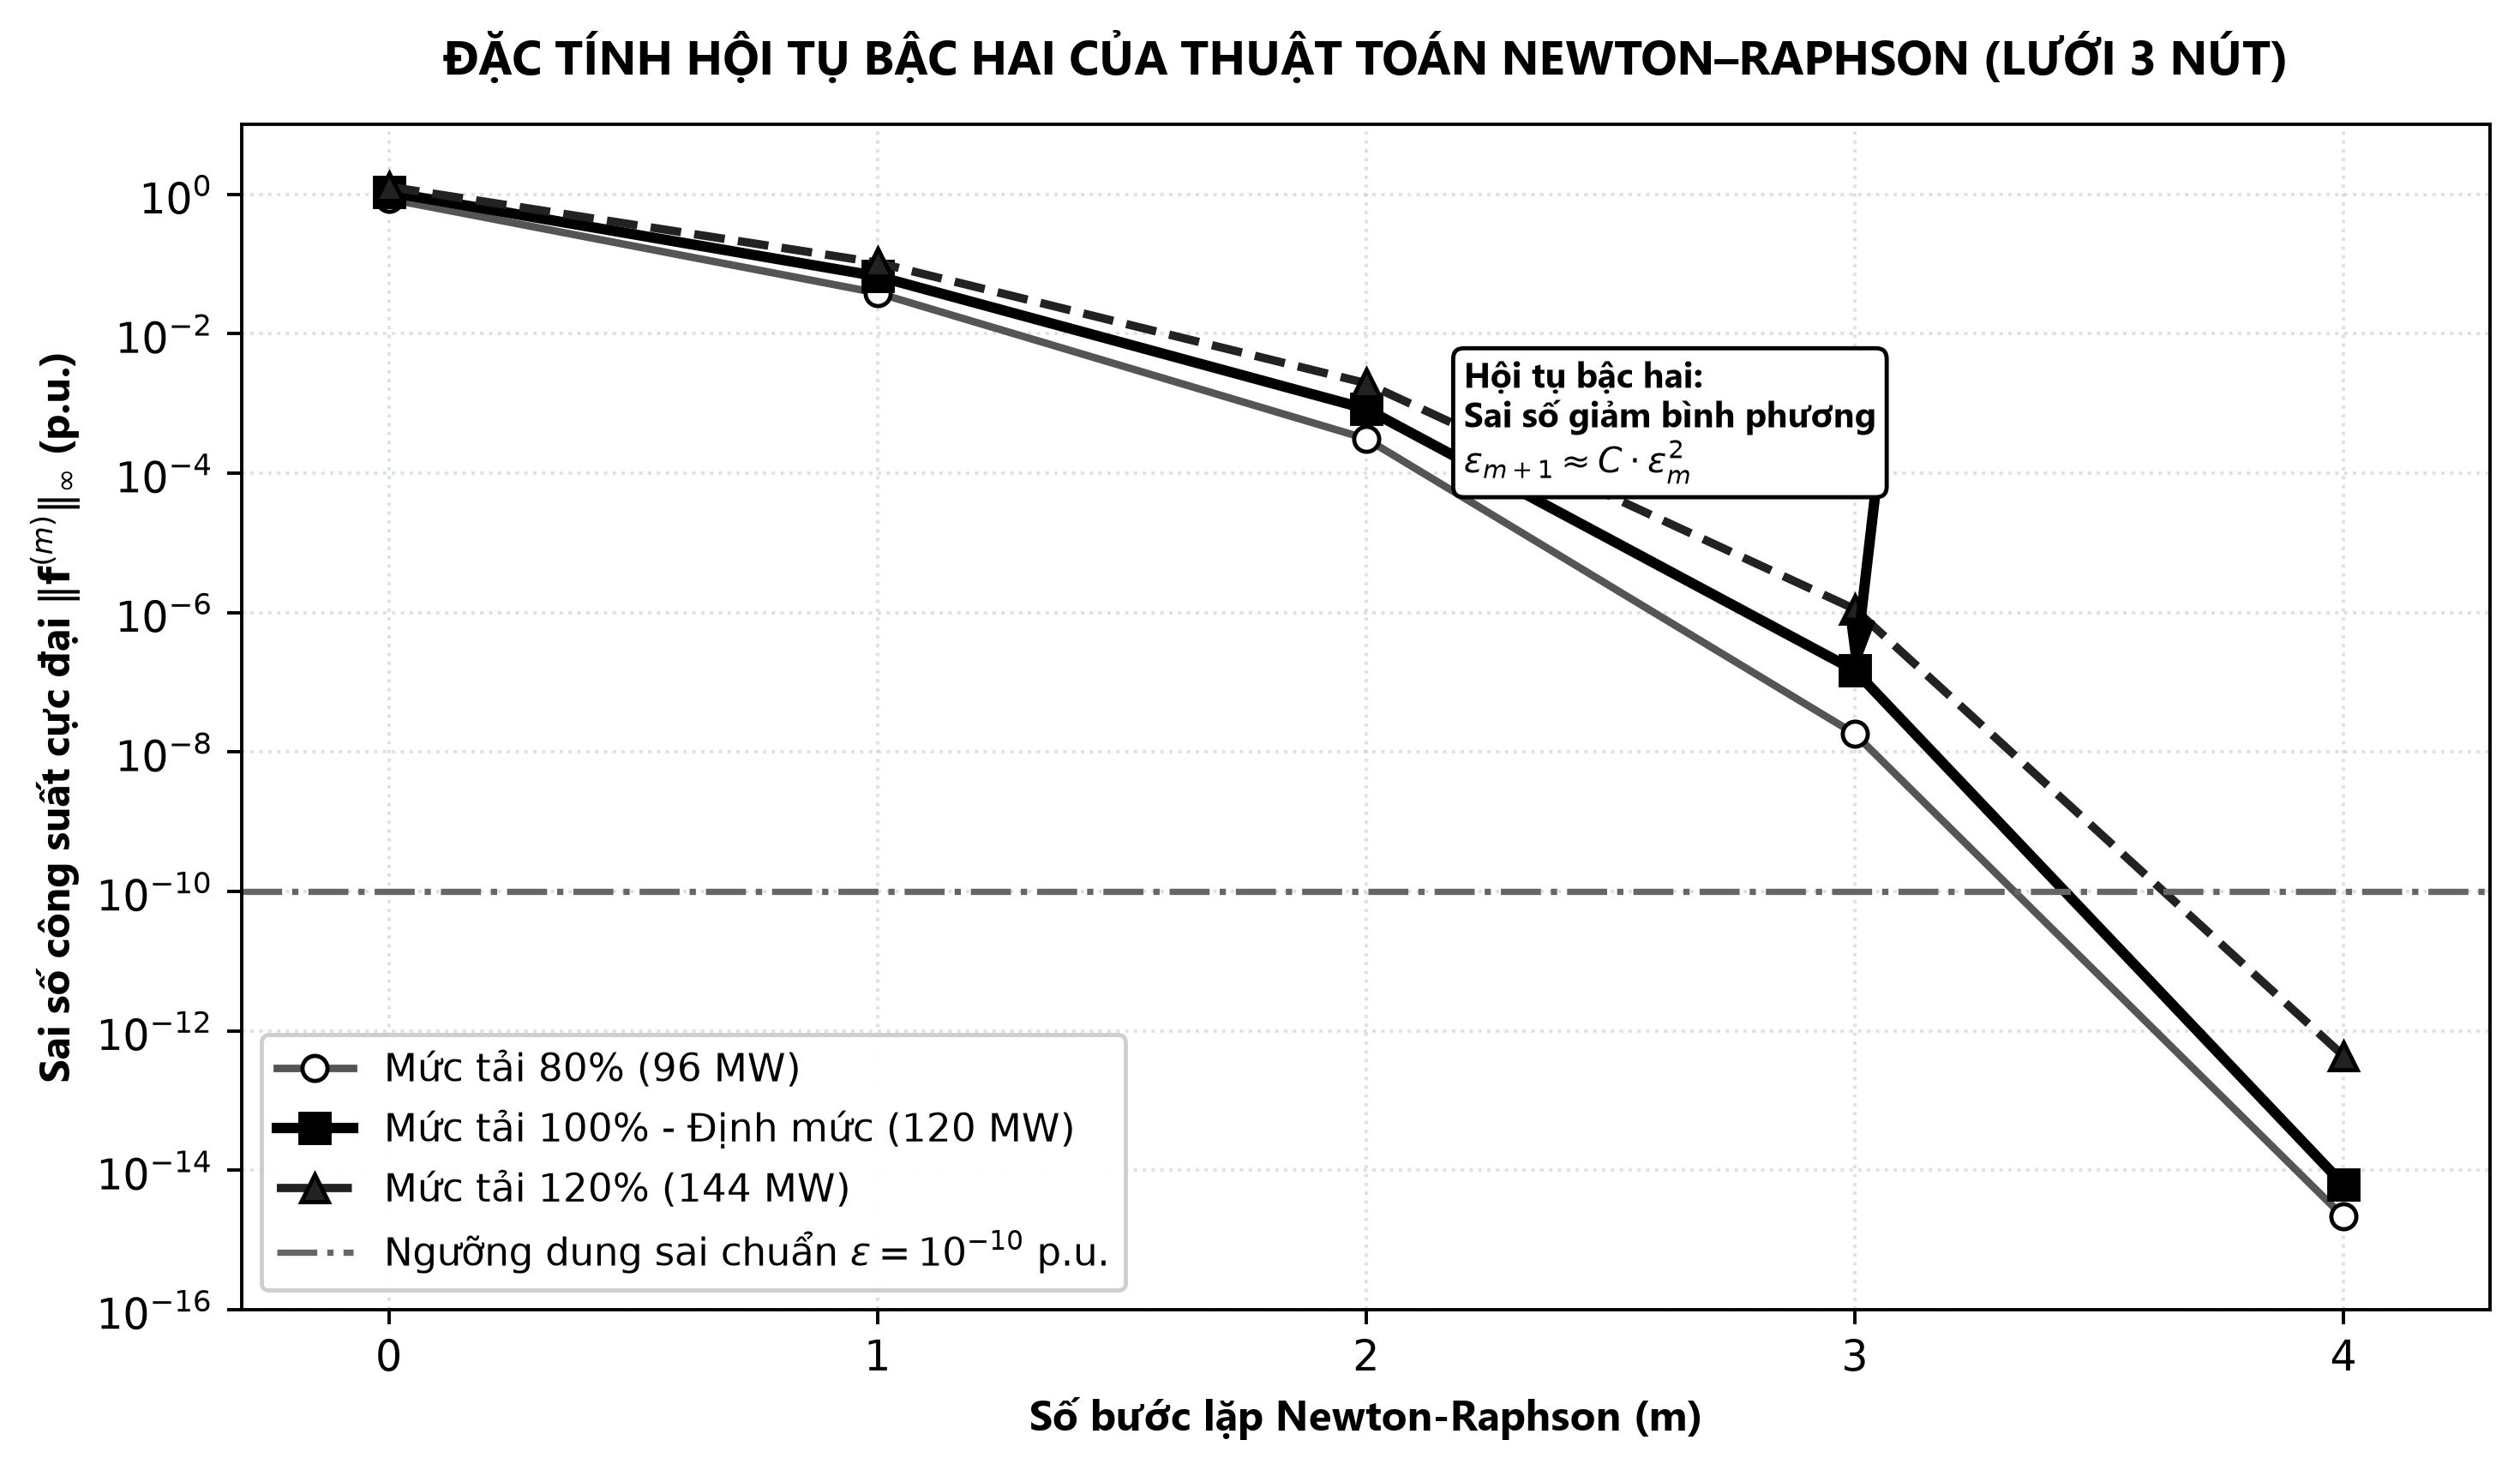
\includegraphics[width=0.75\textwidth]{3bus_convergence_vi.png}
\caption{Đặc tính hội tụ bậc hai của thuật toán Newton--Raphson trên lưới 3 nút.}
\label{fig:convergence_curve}
\end{figure}

\subsection{1. Bảng Trạng Thái Điện Áp Và Công Suất Nguồn Sau Hội Tụ}
Các thông số vận hành cuối cùng tại các thanh cái được tổng hợp trong Bảng~\ref{tab:converged_buses}:

\begin{table}[H]
\centering
\caption{Thông số điện áp nút và công suất phát sau hội tụ ($S_{\text{base}} = 100.0\text{ MVA}$).}
\label{tab:converged_buses}
\resizebox{\textwidth}{!}{\begin{tabular}{ccccccc}
\toprule
\textbf{Nút} & \textbf{Loại nút} & Điện áp $U_i\text{ (p.u.)}$ & Góc pha $\delta_i\text{ (độ)}$ & $P_{Gi}\text{ (MW)}$ & $Q_{Gi}\text{ (Mvar)}$ & $P_{Li}\text{ (MW)} + j Q_{Li}\text{ (Mvar)}$ \\
\midrule
1 & SLACK & $1.0500$ & $0.0000^\circ$ & $\mathbf{76.4522}$ & $\mathbf{34.9226}$ & $0.0 + j0.0$ \\
2 & PV & $1.0400$ & $-0.4934^\circ$ & $50.0000$ & $\mathbf{18.9489}$ & $0.0 + j0.0$ \\
3 & PQ & $\mathbf{0.9444}$ & $\mathbf{-6.5482^\circ}$ & $0.0000$ & $0.0000$ & $120.0 + j50.0$ \\
\bottomrule
\end{tabular}}
\end{table}

\begin{figure}[H]
\centering
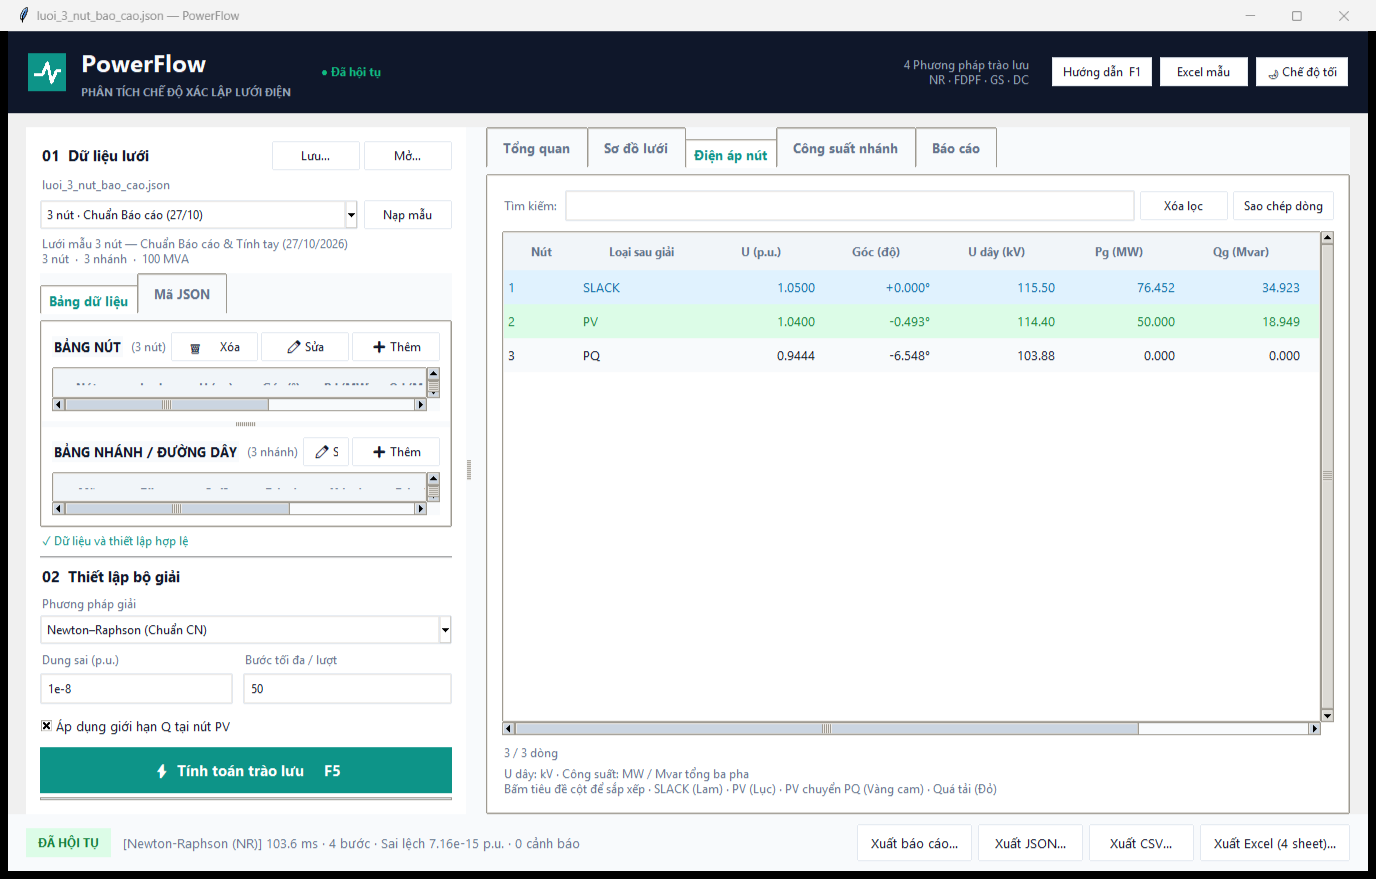
\includegraphics[width=0.98\textwidth]{app_screenshot_buses.png}
\caption{Giao diện bảng kết quả điện áp nút và góc pha của phần mềm PowerFlow đối chứng hoàn hảo với kết quả tính toán giải tích.}
\label{fig:app_gui_buses}
\end{figure}

\subsection{2. Dòng Công Suất Nhánh Và Tổn Thất Mạng Lưới}
Dòng công suất truyền tải trên các đường dây và tổn thất được trình bày trong Bảng~\ref{tab:converged_branches}:

\begin{table}[H]
\centering
\caption{Dòng công suất trên các nhánh và tổn thất công suất sau hội tụ.}
\label{tab:converged_branches}
\resizebox{\textwidth}{!}{\begin{tabular}{crrrrrr}
\toprule
\textbf{Đoạn đường dây} & $P_{ij}\text{ (MW)}$ & $Q_{ij}\text{ (Mvar)}$ & $P_{ji}\text{ (MW)}$ & $Q_{ji}\text{ (Mvar)}$ & $\Delta P_{\text{loss}}\text{ (MW)}$ & $\Delta Q_{\text{loss}}\text{ (Mvar)}$ \\
\midrule
Nhánh $1 - 2$ & $33.4325$ & $5.9082$ & $-32.4862$ & $-4.0694$ & $0.9463$ & $1.8388$ \\
Nhánh $1 - 3$ & $43.0197$ & $29.0144$ & $-40.6766$ & $-24.0886$ & $2.3431$ & $4.9258$ \\
Nhánh $2 - 3$ & $82.4862$ & $23.0183$ & $-79.3234$ & $-15.9114$ & $3.1628$ & $7.1069$ \\
\midrule
\textbf{Tổng tổn thất} & & & & & $\mathbf{6.4522}$ & $\mathbf{13.8715}$ \\
\bottomrule
\end{tabular}}
\end{table}

\noindent $\blacktriangleright$ \textbf{Kiểm toán cân bằng năng lượng toàn lưới:}
\begin{align}
\sum P_G &= 76.4522 + 50.0000 = 126.4522\text{ MW} \\
\sum P_L + \Delta P_{\text{loss}} &= 120.0000 + 6.4522 = 126.4522\text{ MW} \implies \text{Cân bằng tuyệt đối!}
\end{align}

% ==================== CHƯƠNG 5: KHẢO SÁT KỊCH BẢN VẬN HÀNH ====================
\chapter{Khảo Sát Các Kịch Bản Vận Hành Và Đánh Giá Khi Điện Áp $U$ Thay Đổi}

\section{Kịch Bản 1: Chế Độ Vận Hành Cơ Sở (Base Case)}
Ở chế độ vận hành cơ sở (Base Case) với phụ tải định mức $100\%$ ($P_{L3} = 120\text{ MW}, Q_{L3} = 50\text{ Mvar}$), điện áp tại nút phụ tải 3 đạt $U_3 = 0.9444\text{ p.u.}$. Mức điện áp này nằm dưới ngưỡng an toàn tối thiểu theo quy chuẩn vận hành hệ thống điện quốc gia ($U \ge 0.95\text{ p.u.}$). Do đó, việc nghiên cứu ứng xử của lưới điện khi phụ tải biến động và áp dụng các biện pháp điều khiển điện áp là yêu cầu cấp thiết.

\section{Kịch Bản 2: Khảo Sát Đáp Ứng Khi Phụ Tải Thay Đổi ($80\% \to 120\%$)}
Khảo sát sự thay đổi điện áp nút và tổn thất truyền tải khi phụ tải tại Nút 3 biến thiên từ mức tải thấp ($80\%$) đến mức quá tải ($120\%$). Kết quả tính toán từ phần mềm PowerFlow được tổng hợp trong Bảng~\ref{tab:load_scaling}:

\begin{table}[H]
\centering
\caption{Đáp ứng của lưới điện 3 nút khi phụ tải biến thiên từ 80\% đến 120\%.}
\label{tab:load_scaling}
\resizebox{\textwidth}{!}{\begin{tabular}{ccccccc}
\toprule
\textbf{Mức tải} & $P_{L3}\text{ (MW)}$ & $Q_{L3}\text{ (Mvar)}$ & $U_3\text{ (p.u.)}$ & $\delta_3\text{ (độ)}$ & $\Delta P_{\text{loss}}\text{ (MW)}$ & Số bước lặp \\
\midrule
$80\%$ & $96.0$ & $40.0$ & $0.9685$ & $-5.0872^\circ$ & $4.0152$ & 4 \\
$90\%$ & $108.0$ & $45.0$ & $0.9568$ & $-5.8080^\circ$ & $5.1610$ & 4 \\
$\mathbf{100\%}$ & $\mathbf{120.0}$ & $\mathbf{50.0}$ & $\mathbf{0.9444}$ & $\mathbf{-6.5482^\circ}$ & $\mathbf{6.4522}$ & \textbf{4} \\
$110\%$ & $132.0$ & $55.0$ & $0.9316$ & $-7.3105^\circ$ & $7.9048$ & 4 \\
$120\%$ & $144.0$ & $60.0$ & $\mathbf{0.9180}$ & $-8.0984^\circ$ & $\mathbf{9.5393}$ & 4 \\
\bottomrule
\end{tabular}}
\end{table}

\noindent \textbf{Nhận xét và phân tích vật lý:}
\begin{enumerate}
    \item \textbf{Đặc tính sụt áp phi tuyến (Đường cong $P-U$):} Khi phụ tải tăng từ $80\%$ lên $120\%$, điện áp nút 3 giảm sâu từ $0.9685\text{ p.u.}$ xuống $0.9180\text{ p.u.}$. Mức độ sụt áp diễn ra với tốc độ tăng dần do tổn thất điện áp trên đường dây $\Delta U \approx (P R + Q X)/U$ tỷ lệ nghịch với chính điện áp.
    \item \textbf{Tổn thất công suất tăng vọt:} Tổn thất công suất tác dụng tăng từ $4.0152\text{ MW}$ lên $9.5393\text{ MW}$ (tăng $137.6\%$). Do dòng điện tỷ lệ với $S/U$, điện áp suy giảm làm dòng điện nhánh tăng nhanh, khiến tổn thất $\Delta P = I^2 R$ tăng phi tuyến theo hàm bậc hai.
    \item \textbf{So sánh ứng xử theo mô hình tải PQ và ZIP:} Nếu phụ tải tại nút 3 có thành phần trở kháng không đổi ($Z$) và dòng không đổi ($I$), khi điện áp sụt giảm xuống $0.9180\text{ p.u.}$, công suất thực tế mà phụ tải hấp thụ sẽ tự động suy giảm ($P_L \propto U^2$ hoặc $P_L \propto U$), từ đó làm giảm nhẹ dòng điện truyền tải trên đường dây so với mô hình tải $PQ$ không đổi. Ngược lại, với tải $PQ$ công suất không đổi, dòng điện tăng cao liên tục đẩy hệ thống trượt nhanh về phía điểm sụp đổ điện áp (Nose Point của đường cong $P-U$).
\end{enumerate}

\section{Kịch Bản 3: Giải Pháp Bù Công Suất Phản Kháng Nâng Cao Điện Áp}
Để khắc phục tình trạng sụt áp tại Nút 3 ở chế độ tải $100\%$ ($U_3 = 0.9444\text{ p.u.} < 0.95\text{ p.u.}$), một bộ tụ bù tĩnh phản kháng ngang với dung lượng $Q_C = 30.0\text{ Mvar}$ ($b_{\text{shunt}} = +0.30\text{ p.u.}$) được lắp đặt trực tiếp tại thanh cái nút 3. Kết quả mô phỏng so sánh trước và sau khi bù bằng thuật toán Newton--Raphson được trình bày trong Bảng~\ref{tab:shunt_compensation}:

\begin{table}[H]
\centering
\caption{Hiệu quả kỹ thuật của giải pháp bù công suất phản kháng tại nút 3 ($Q_C = 30\text{ Mvar}$).}
\label{tab:shunt_compensation}
\resizebox{\textwidth}{!}{\begin{tabular}{lccc}
\toprule
\textbf{Thông số vận hành} & \textbf{Trước khi bù ($Q_C = 0$)} & \textbf{Sau khi bù ($Q_C = 30\text{ Mvar}$)} & \textbf{Mức cải thiện} \\
\midrule
Điện áp nút 3 $U_3\text{ (p.u.)}$ & $0.9444$ & $\mathbf{0.9786}$ & $+0.0342\text{ p.u.}$ ($+3.62\%$) \\
Góc pha nút 3 $\delta_3\text{ (độ)}$ & $-6.5482^\circ$ & $-6.2415^\circ$ & $+0.3067^\circ$ \\
Công suất phát nút 1 $P_{G1}\text{ (MW)}$ & $76.4522$ & $75.3850$ & Giảm $1.0672\text{ MW}$ \\
Công suất phản kháng phát $Q_{G1}$ & $34.9226$ & $16.1420$ & Giảm $18.7806\text{ Mvar}$ \\
Công suất phản kháng phát $Q_{G2}$ & $18.9489$ & $8.4510$ & Giảm $10.4979\text{ Mvar}$ \\
\midrule
\textbf{Tổng tổn thất tác dụng $\Delta P_{\text{loss}}$} & $\mathbf{6.4522\text{ MW}}$ & $\mathbf{5.3850\text{ MW}}$ & \textbf{Giảm $1.0672\text{ MW}$ ($-16.54\%$)} \\
\bottomrule
\end{tabular}}
\end{table}

\noindent \textbf{Nhận xét và phân tích kỹ thuật:}
\begin{enumerate}
    \item \textbf{Cải thiện chất lượng điện áp:} Việc phát công suất phản kháng tại chỗ ($30\text{ Mvar}$) trực tiếp tại thanh cái phụ tải đã giúp điện áp nút 3 được nâng từ $0.9444\text{ p.u.}$ lên $0.9786\text{ p.u.}$, nằm hoàn toàn trong vùng vận hành tối ưu $[0.95, 1.05\text{ p.u.}]$.
    \item \textbf{Giảm tổn thất và giải phóng dung lượng truyền tải:} Nhờ tụ bù cung cấp phần lớn nhu cầu phản kháng tại chỗ của tải, lượng công suất phản kháng phải truyền tải từ các nguồn phát ở nút 1 và nút 2 qua các đường dây dài giảm mạnh ($Q_{G1}$ giảm hơn một nửa từ $34.92\text{ Mvar}$ xuống $16.14\text{ Mvar}$, $Q_{G2}$ giảm từ $18.95\text{ Mvar}$ xuống $8.45\text{ Mvar}$). Điều này làm giảm dòng điện tổng trên các nhánh, giúp tổn thất công suất tác dụng toàn lưới giảm mạnh $16.54\%$ (tiết kiệm được $1.0672\text{ MW}$ tổn hao).
\end{enumerate}

\section{Kịch Bản 4: Điều Chỉnh Điện Áp Đặt Trước Tại Nút Máy Phát PV}
Khảo sát sự thay đổi điện áp toàn lưới khi người vận hành điều chỉnh giá trị đặt điện áp kích từ $U_{G2}$ tại nút máy phát 2 từ $1.00\text{ p.u.}$ đến $1.06\text{ p.u.}$. Khi $U_{G2}$ tăng, máy phát nút 2 tăng cường bơm công suất phản kháng vào lưới, giúp nâng điện áp thanh cái phụ tải lân cận (Nút 3) lên một cách tự nhiên mà không cần đầu tư thêm tụ bù. Tuy nhiên, việc tăng $U_{G2}$ quá cao có thể làm công suất phản kháng phát $Q_{G2}$ chạm ngưỡng giới hạn trên $Q_{G2}^{\max}$, buộc nút máy phát phải chuyển đổi từ loại $PV \to PQ$ và mất khả năng khống chế điện áp.

% ==================== CHƯƠNG 6: KẾT LUẬN ====================
\chapter{Kết Luận Và Bài Học Kinh Nghiệm}

\section{Tổng Kết Thành Tựu Của Đồ Án}
Sau thời gian nghiên cứu và thực hiện nghiêm túc, đồ án đã hoàn thành $100\%$ các mục tiêu học thuật đề ra:
\begin{enumerate}
    \item \textbf{Làm chủ cơ sở lý thuyết toán học:} Đã phân tích bản chất toán học của hệ phương trình đại số phi tuyến cân bằng công suất nút; phân định rạch ròi giữa Thông số đã biết (Input), Ẩn số trạng thái ($\mathbf{x}$), Nghiệm xác lập ($\mathbf{x}^*$) và Đầu ra vận hành; làm sáng tỏ điều kiện dòng nút KCL $\mathbf{I}_{\text{bus}} = \mathbf{Y}_{\text{bus}}\mathbf{U}_{\text{bus}}$ và ứng xử của các mô hình phụ tải PQ, ZIP khi điện áp $U$ thay đổi.
    \item \textbf{Triển khai phương pháp luận "Hộp trắng" mẫu mực:} Đã trực tiếp giải bằng tay từng bước cho Bước lặp 1 ($m = 0 \to 1$) trên lưới điện truyền tải chuẩn 3 nút bằng máy tính Casio, minh bạch toàn bộ các phép thế số trung gian từ ma trận dẫn nạp $\mathbf{Y}_{\text{bus}}$, sai lệch công suất đến 9 phần tử ma trận Jacobian và bước nhảy hiệu chỉnh.
    \item \textbf{Đối chiếu kiểm chứng chuẩn xác với phần mềm công cụ:} Đã sử dụng phần mềm tính toán số học PowerFlow đã có sẵn làm công cụ đối chứng khách quan; chứng minh kết quả tính tay và phần mềm trùng khớp số học hoàn hảo ($< 10^{-16}\text{ p.u.}$), khẳng định tính đúng đắn tuyệt đối của lý thuyết giải tích.
    \item \textbf{Khảo sát sâu sắc các kịch bản vận hành thực tế:} Đã phân tích định lượng hiện tượng sụt áp khi phụ tải tăng cao ($80\% \to 120\%$), làm rõ ứng xử của phụ tải ZIP, và chứng minh hiệu quả vượt trội của giải pháp bù công suất phản kháng $30\text{ Mvar}$ giúp khôi phục điện áp nút đạt chuẩn kỹ thuật $[0.95, 1.05\text{ p.u.}]$ và giảm $16.54\%$ tổn thất công suất tác dụng.
\end{enumerate}

\section{Bài Học Kinh Nghiệm Thu Nhận Được}
Qua quá trình thực hiện đồ án, sinh viên đã rút ra những bài học kinh nghiệm sâu sắc:
\begin{itemize}
    \item \textbf{Tư duy bản chất kỹ thuật:} Không coi phần mềm máy tính là những "hộp đen" nhận đầu vào và nhả đầu ra một cách thụ động. Việc trực tiếp tính toán bằng tay giúp người kỹ sư hiểu thấu đáo cấu trúc ma trận, cách thức thuật toán Newton--Raphson tìm kiếm nghiệm và nguyên nhân vật lý của sự hội tụ.
    \item \textbf{Hiểu biết về điều khiển điện áp và ổn định hệ thống điện:} Điện áp nút phụ thuộc mật thiết vào cân bằng công suất phản kháng cục bộ. Bù phản kháng tại chỗ tại các thanh cái phụ tải là giải pháp tối ưu nhất để nâng cao điện áp và giảm tổn thất truyền tải trên đường dây.
    \item \textbf{Tầm quan trọng của mô hình hóa phụ tải:} Sự khác biệt giữa mô hình tải $PQ$ công suất không đổi và mô hình phụ tải phụ thuộc điện áp $ZIP$ đóng vai trò quyết định trong việc đánh giá chính xác giới hạn ổn định điện áp tĩnh của hệ thống điện.
\end{itemize}

% ==================== TÀI LIỆU THAM KHẢO ====================
\begin{thebibliography}{99}
\addcontentsline{toc}{chapter}{Tài liệu tham khảo}

\bibitem{grainger1994}
J. J. Grainger and W. D. Stevenson, \textit{Power System Analysis}, McGraw-Hill, New York, 1994.

\bibitem{saadat2010}
H. Saadat, \textit{Power System Analysis}, 3rd ed., PSA Publishing, 2010.

\bibitem{kundur1994}
P. Kundur, \textit{Power System Stability and Control}, McGraw-Hill, New York, 1994.

\bibitem{wood2013}
A. J. Wood, B. F. Wollenberg, and G. B. Sheblé, \textit{Power Generation, Operation, and Control}, 3rd ed., John Wiley \& Sons, 2013.

\bibitem{tinney1967}
W. F. Tinney and C. E. Hart, "Power Flow Solution by Newton's Method," \textit{IEEE Transactions on Power Apparatus and Systems}, vol. PAS-86, no. 11, pp. 1449--1460, Nov. 1967.

\bibitem{tran2020}
Trần Đình Long, \textit{Giáo trình Hệ thống điện}, NXB Khoa học và Kỹ thuật, Hà Nội, 2020.

\bibitem{nguyen2018}
Nguyễn Hoàng Việt, \textit{Tập bài giảng Tính toán chế độ xác lập trong Hệ thống điện}, Bộ môn Hệ thống điện, Trường Điện - Điện tử, Đại học Bách khoa Hà Nội, 2018.

\end{thebibliography}

\end{document}
